%%%%%%%%%%%%%%%%%%%%%%%%%%%%%%%%%%%%%%%%%%%%%%%%%%%%%%%%%%%%%%%%%%%%
%%%%%%%%%%%%%%%%%%%%%%%%%%%%%%%%%%%%%%%%%%%%%%%%%%%%%%%%%%%%%%%%%%%%
%%                                                                %%
%% An example for writting your thesis using LaTeX                %%
%% Original version by Luis Costa,  changes by Perttu Puska       %%
%% Support for Swedish added 15092014                             %%
%%                                                                %%
%% This example consists of the files                             %%
%%         thesistemplate.tex (versio 2.01)                       %%
%%         opinnaytepohja.tex (versio 2.01) (for text in Finnish) %%
%%         aaltothesis.cls (versio 2.01)                          %%
%%         kuva1.eps                                              %%
%%         kuva2.eps                                              %%
%%         kuva1.pdf                                              %%
%%         kuva2.pdf                                              %%
%%                                                                %%
%%                                                                %%
%% Typeset either with                                            %%
%% latex:                                                         %%
%%             $ latex opinnaytepohja                             %%
%%             $ latex opinnaytepohja                             %%
%%                                                                %%
%%   Result is the file opinnayte.dvi, which                      %%
%%   is converted to ps format as follows:                        %%
%%                                                                %%
%%             $ dvips opinnaytepohja -o                          %%
%%                                                                %%
%%   and then to pdf as follows:                                  %%
%%                                                                %%
%%             $ ps2pdf opinnaytepohja.ps                         %%
%%                                                                %%
%% Or                                                             %%
%% pdflatex:                                                      %%
%%             $ pdflatex opinnaytepohja                          %%
%%             $ pdflatex opinnaytepohja                          %%
%%                                                                %%
%%   Result is the file opinnaytepohja.pdf                        %%
%%                                                                %%
%% Explanatory comments in this example begin with                %%
%% the characters %%, and changes that the user can make          %%
%% with the character %                                           %%
%%                                                                %%
%%%%%%%%%%%%%%%%%%%%%%%%%%%%%%%%%%%%%%%%%%%%%%%%%%%%%%%%%%%%%%%%%%%%
%%%%%%%%%%%%%%%%%%%%%%%%%%%%%%%%%%%%%%%%%%%%%%%%%%%%%%%%%%%%%%%%%%%%

%% Uncomment one of these:
%% the 1st when using pdflatex, which directly typesets your document in
%% pdf (use jpg or pdf figures), or
%% the 2nd when producing a ps file (use eps figures, don't use ps figures!).
\documentclass[english,12pt,a4paper,pdftex,elec,utf8,sci]{aaltothesis}
%\documentclass[english,12pt,a4paper,dvips]{aaltothesis}

%% To the \documentclass above
%% specify your school: arts, biz, chem, elec, eng, sci
%% specify the character encoding scheme used by your editor: utf8, latin1

%% Use one of these if you write in Finnish (see the Finnish template):
%%
%\documentclass[finnish,12pt,a4paper,pdftex,elec,utf8]{aaltothesis}
%\documentclass[finnish,12pt,a4paper,dvips]{aaltothesis}

\usepackage{graphicx,wrapfig}

%% Use this if you write hard core mathematics, these are usually needed
\usepackage{amsfonts,amssymb,amsbsy,relsize,amsthm}

%% Use the macros in this package to change how the hyperref package below 
%% typesets its hypertext -- hyperlink colour, font, etc. See the package
%% documentation. It also defines the \url macro, so use the package when 
%% not using the hyperref package.
%%
%\usepackage{url}

%% Use this if you want to get links and nice output. Works well with pdflatex.
\usepackage{hyperref}
\hypersetup{pdfpagemode=UseNone, pdfstartview=FitH,
  colorlinks=true,urlcolor=red,linkcolor=blue,citecolor=black,
  pdftitle={Engineering Multi Electrode Patch Clamp System to Quantify Neural Circuits},pdfauthor={Sathish Kumar Narayanan},
  pdfkeywords={Modify keywords}}


%% All that is printed on paper starts here
\begin{document}

%% Change the school field to specify your school if the automatically 
%% set name is wrong
% \university{aalto-yliopisto}
% \university{aalto University}
% \school{Sähkötekniikan korkeakoulu}
% \school{School of Science}

%% Only for B.Sc. thesis: Choose your degree programme. 
%\degreeprogram{Electronics and electrical engineering}
%%

%% ONLY FOR M.Sc. AND LICENTIATE THESIS: Specify your department,
%% professorship and professorship code. 
%%
\department{Computer Science and Information Science}
\professorship{Machine Learning and Data Mining}
%%

%% Valitse yksi näistä kolmesta
%%
%% Choose one of these:
%\univdegree{BSc}
\univdegree{MSc}
%\univdegree{Lic}

%% Your own name (should be self explanatory...)
\author{Sudhanshu Nautiyal}

%% Your thesis title comes here and again before a possible abstract in
%% Finnish or Swedish . If the title is very long and latex does an
%% unsatisfactory job of breaking the lines, you will have to force a
%% linebreak with the \\ control character. 
%% Do not hyphenate titles.
%% 
\thesistitle{Multi-trial classification using latent Gaussian Processes}

\place{Espoo}

%% For B.Sc. thesis use the date when you present your thesis. 
%% 
%% Kandidaatintyön päivämäärä on sen esityspäivämäärä! 
\date{16.1.2015}

%% B.Sc. or M.Sc. thesis supervisor 
%% Note the "\" after the comma. This forces the following space to be 
%% a normal interword space, not the space that starts a new sentence. 
%% This is done because the fullstop isn't the end of the sentence that
%% should be followed by a slightly longer space but is to be followed
%% by a regular space.
%%
\supervisor{Prof.\ Samual Kaski} %{Prof.\ Pirjo Professori}

%% B.Sc. or M.Sc. thesis advisors(s). You can give upto two advisors in
%% this template. Check with your supervisor how many official advisors
%% you can have.
%%
%\advisor{Prof.\ Petri Ala-Laurila}
\advisor{M.Sc.\ Sami Remes}

%% Aalto logo: syntax:
%% \uselogo{aaltoRed|aaltoBlue|aaltoYellow|aaltoGray|aaltoGrayScale}{?|!|''}
%%
%% Logo language is set to be the same as the document language.
%% Logon kieli on sama kuin dokumentin kieli
%%
\uselogo{aaltoRed}{''}

%% Create the coverpage
%%
\makecoverpage


%% Note that when writting your master's thesis in English, place
%% the English abstract first followed by the possible Finnish abstract

%% English abstract.
%% All the information required in the abstract (your name, thesis title, etc.)
%% is used as specified above.
%% Specify keywords
%%
%% Kaikki tiivistelmässä tarvittava tieto (nimesi, työnnimi, jne.) käytetään
%% niin kuin se on yllä määritelty.
%% Avainsanat
%%
\keywords{For keywords choose concepts that are central to your thesis}
%% Abstract text
\begin{abstractpage}[english]
WIP
\end{abstractpage}

%% Force a new page so that the possible English abstract starts on a new page
%%
%% Pakotetaan uusi sivu varmuuden vuoksi, jotta 
%% mahdollinen suomenkielinen ja englanninkielinen tiivistelmä
%% eivät tule vahingossakaan samalle sivulle
\newpage

%% Preface
%%
%% Esipuhe 
\mysection{Preface}
I want to thank Professor  <> .\\

\vspace{5cm}
Otaniemi, 16.1.2015

\vspace{5mm}
{\hfill Sudhanshu Nautiyal \hspace{1cm}}

%% Force new page after preface
%%
%% Pakotetaan varmuuden vuoksi esipuheen jälkeinen osa
%% alkamaan uudelta sivulta
\newpage


%% Table of contents. 
\thesistableofcontents


%% Symbols and abbreviations
\mysection{Symbols and abbreviations}

\subsection*{Symbols}

\begin{tabular}{ll}
$\mathbf{B}$  & magnetic flux density  \\
$c$              & speed of light in vacuum $\approx 3\times10^8$ [m/s]\\
$\omega_{\mathrm{D}}$    & Debye frequency \\
$\omega_{\mathrm{latt}}$ & average phonon frequency of lattice \\
$\uparrow$       & electron spin direction up\\
$\downarrow$     & electron spin direction down
\end{tabular}

\subsection*{Operators}

\begin{tabular}{ll}
$\nabla \times \mathbf{A}$              & curl of vectorin $\mathbf{A}$\\
$\displaystyle\frac{\mbox{d}}{\mbox{d} t}$ & derivative with respect to 
variable $t$\\[3mm]
$\displaystyle\frac{\partial}{\partial t}$  & partial derivative with respect 
to variable $t$ \\[3mm]
$\sum_i $                       & sum over index $i$\\
$\mathbf{A} \cdot \mathbf{B}$    & dot product of vectors $\mathbf{A}$ and 
$\mathbf{B}$
\end{tabular}

\subsection*{Abbreviations}

\begin{tabular}{ll}
AC         & alternating current \\
APLAC      & an object-oriented analog circuit simulator and design tool \\
           & (originally Analysis Program for Linear Active Circuits) \\
BCS        & Bardeen-Cooper-Schrieffer \\ %% dash between the names
DC         & direct current \\
TEM        & transverse eletromagnetic
\end{tabular}


%% Tweaks the page numbering to meet the requirement of the thesis format:
%% Begin the pagenumbering in Arabian numerals (and leave the first page
%% of the text body empty, see \thispagestyle{empty} below).
%% Additionally, force the actual text to begin on a new page with the 
%% \clearpage command.
%% \clearpage is similar to \newpage, but it also flushes the floats (figures
%% and tables).
%% There is no need to change these
%%
\cleardoublepage
\storeinipagenumber
\pagenumbering{arabic}
\setcounter{page}{1}




\section{Introduction [WIP]}
\clearpage
\section{Background}
A typical statistical inference problem usually deals with estimation of unknown quantities based on some observed information. Due to their many desirable qualities like ability to provide uncertainty around the estimations, seamless incorporation of new information to the model and elimination, Bayesian methodology has considerable advantage over other approaches to data analysis and statistical inference. In this section we briefly review the bayesian inference and then explore inference problem from a non parametric perspective. Section 2.2 further provides a introduction to Gaussian Processes as a bayesian non parametric method and finally a short overview of sparse approximation technique is provided in section 2.2.3

\subsection{Bayesian Inference}

Bayesian methods approach the solution of inference problem from a probabilistic perspective by setting up a model that constitutes our assumptions and knowledge about all relevant observed as well as unobserved quantities as probabilistic statements. 
The complete inference process then consists of three steps, First formulation of initial knowledge about the model and its constituents in terms of prior and joint distribution. Bayes’ theorem is then used to figure out the posterior - conditional probability distribution of unobserved quantities given the observed ones. This posterior distribution is considered to be the underlying distribution from which all unobserved quantities were generated in the past and will continue to do so in future. Finally, a formal validation step can be performed to determine model’s ability to explain the observations and thereby its correctness[BDA, A gelmen].
Thus in a generic Bayesian analysis process, parameters describe the particular data generating model we believe the observations arose from and the inference process becomes about finding the possible values of parameters that could generate the given observations:
\begin{equation}
\scriptstyle
P(parameters | observation, model) =  P(observations | parameters, model) P(parameters,model)
\end{equation}

Here the first term at RHS tells us the probability of seeing those observations given a particular set of parameters i.e. likelihood and the second term incorporates our belief about those parameter values before seeing the observations, i.e. prior.
Once the posterior is identified, that means models and its parameters have been recognized one could either generate or predict new data:

\begin{equation}
\scriptstyle
    P(x| parameters, observation,model) = \integration P(x | parameters , observation, model) P(parameters |observation, model)
    \label{eqn:general_margin}
\end{equation}

\subsubsection{Parametric and Non Parametric Models}

Based on the specific problem at hand, we usually make certain assumptions about the model. These salient properties of model are included in the inference process as the model parameters. For example, its common to assume sampling distribution of a continuous quantity to be normal. In that case mean and variance would be termed as model parameters. Similarly, number of clusters would be a parameter in case of a mixture model. The specific parameters value then can be used describe that particular model. Once the value of these parameters are known, the model is said to be identified, i.e. complete knowledge about observed data and its generating process is transferred in the parameters from observations. From the perspective of equation \ref{eqn:general_margin}, 
 $$P(x| parameters, data, model) =  P(x| parameters, model)$$
Or in other words, parameters have extracted ‘everything there was to know about data releavent to future predicitons’ [http://mlg.eng.cam.ac.uk/pub/pdf/Gha12.pdf.] 

However, this requirement of making initial assumption about parameters means for parametric mdoels underlying distribution is restricted to be in the same category as the other models with similar parameterization. [O’Hagan book] This restriction as we will see later makes these models inflexible and of limited capacity. 

Conversely, in cases where we want to make no assumptions to restrict the model we stipulate a generic model with no fixed number of parameters and call them non-parametric models. A non parametric regression model for example would not consider any specific function form but just a collection of functions one of which might have generated the observations. 

Since the model is considered to be the process that generated the observational data during data analysis, another way to look at the distinction between parametric and non parametric is by considering our model to be a subset of the set of all data generating processes defined in a parameter space that is indexed by a vector of model parameters. A parametric model then will have a finite length parameter vector identifying a subset of data generating process while non parametric model will have infinite number of parameters representing unrestricted amount of models that can be considered (Figure \ref{fig:generic_function_space}). 
\begin{figure}
    \centering
    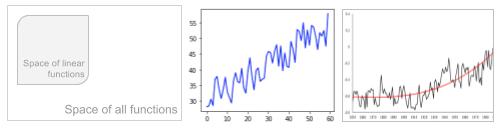
\includegraphics[scale=0.75]{thesis/images/function_spaces.png}
    \caption{Left: Illustration of function spaces and linear spaces with in it, Middle: A linear trend, Right: Non Linear trend}
    \label{fig:generic_function_space}
\end{figure}
Apart from possibility to consider a richer set of models by making minimal assumptions, non parametric models also provide a coherent way of model criticism and prior selection. In Bayesian analysis, the prior beliefs used to derive posterior must represent the actual state of knowledge without the knowledge of observations. Thus, the model selection approach to alleviate prior uncertainty by first using multiple priors and then selecting one of them based on the most convincing posterior results (after looking at the observation) is not considered coherent, specially in Bayesian paradigms where appropriately used methods should not overfit any ways [http://www.gatsby.ucl.ac.uk/~edward/pub/occam.pdf, Mackay 91] A non parametric approach on the other hand goes around models selection issue due to its ability to specify unrestricted forms can be used to accommodate the uncertainty around priors [Bayesian Non Paramterics book].

This problem of choosing a model’s parameters beforehand or model selection has prime importance in machine learning arena. Improper model selection significantly impacts a model’s performance through generating an over or under fitted model. Moreover, some use cases where identification of underlying structure of data is important like hidden Markov models, mixture models etc., might require one to supply the parameters even before the inference process has begun. Usual solution to these model selection issues is to perform cross validation [reference missing]. However, depending upon the situation it might either be inefficient to compare all the possible models or simply incoherent from Bayesian perspective as explained in the previous paragraph to reuse data multiple times. Bayesian Nonparametric methods gets around this problem by adapting the complexity of model based on available data, [Baysian nonparametric methods paper] i.e allowing for gradually more complex model as the amount of data grows. For example, a traditional mixture model requires number of clusters to be fixed before hand while non parametric approach would be able to infer even the number of clusters from the data and allows it to increase as it encounters new data. [Chinese buffet process, drichlet process article]

\subsubsection{Non parametric models}

In most machine learning application our objective is to find a ‘pattern’ that can be used to explain observed data. In most cases a function can be used to represent this pattern and thus our objective becomes to search for the function among many possible functions that best explains the data. However, we might reduce the search space by making some common sense assumptions. For example, to find the function that explain clearly linear data in Figure \ref{fig:generic_function_space}(middle) one might want to search within smooth linear function spaces while in case of Figure \ref{fig:generic_function_space}(right) we would like to relax the linear constraint and search among all possible smooth functions.  As can be observed, this is analogous to putting prior over parameters in Bayesian analysis but now parameter space represents all possible functions and prior encapsulates our initial guess about the space where our viable solution should exist. 

It is clear form above discussion that Bayesian nonparametric model requires us to put probability distribution over these functions (infinite dimensional objects). Beginning from Fergusson’s work on Drichlet’s processes [T. Fergusson 1973] various strategies have been recommended to build these models. [Neil, 2005] for example recommends starting from a parametric model and then take infinite limit of it. Due to their propensity to work with infinite dimensional objects, a lot of work in this field have been done under stochastic process analysis. Historically Drichlet process  and Gaussian processes have dominated the nonparametric models. Drichlet’s process is sued to put distribution over distributions and hence has been primarily used in relation to density estimation or topic modelling related problem[Reference to Ferguson paper and other DP papers]. Gaussian Processes are another famous tool set that have been used extensively to solve Bayesian nonparametric problems where funcitons are to be estimated, i.e. putting distributions over functions. Next section explores Gaussian processes in more detail.








\subsection{Gaussian Processes}
Due to their seemingly simple nature and interesting analytical properties Gaussian processes have been used extensively in various tasks for centuries. Flexibility of Gaussian Processes have seen them employed in various forms. [BDA reference about 1800 century], Gelmen et al. mention them being used for astronomical data modelling in 18th century. Later, significant work have been done as part of stochastic process literature for example as Weiner processes and later for time series prediction[Weiner process, A Populi’91 reference for stochastic process and other Reference from Phd thesis]. In Spatial statistics, gaussian process regression was used for interpolation of values based on space as the input by Matheron in 1973 following the work of D.G. Krige [ both references from wiki]. In applied statistics context, Gaussian processes were first used for regression and classification [O’Hagan 1978], density estimation [reference from BDA, rihimaki thesis and other one ] etc. Inspired by the link shown between neural networks and Gaussian process by [Neal ‘ 96] Gaussian processes were quickly extended to machine learning context[Rasmussen 96]. With the advent of approximation schemes [Sparse approximation referneces] and hardware gains, use of Gaussian process has quickly skyrocketed in other areas of machine learning such as dimensionality reduction [reference], latent vector modelling [reference], even multi purpose deep Gaussian processes analogous to deep neural network have been proposed [GPRN paper, deep GP paper].  In the next few sections, we first define Gaussian processes and review it's properties like covariance functions etc briefly and later describe the inference procedure including  predictions and parameter selection in Section 2.2 
\subsubsection{Definition}
A function is generally thought of as a mapping from an arbitrary set X to another F(X), $X -> F(X)$. One interesting way to look at it can be of thinking X and F(X) as infinitely long vectors with former’s elements acting as an index for the latter, i.e. X as an index set for F(X).  A collection of these random mappings is called a process [Random Fields and geometry, Andler, Stochastic process book]. 

A Gaussian Process is thus formally defined as a collection of random variables, any finite set of which is jointly distributed. i.e. for a finite set x contained in X , collection of random variables F(x) will follow a Gaussian distribution [GPML book], i.e. 

\begin{equation}
    p(F|X) ~ mathbb{N}(m,K)
    \label{eqn:GP_definition}
\end{equation} 

In gaussian process terms f(x) is written as $f(x) ~ GP(m(x),k(x,x))$ where m(x) and k(x,x) are called the mean and covariance function respectively. 

\subsubsection{Covariance functions and Kernels}

From a function perspective, one expects that data points close/near to each other will have similar values. This notion of nearness can also be seen in general life for example, if one were to measure moisture in environment at a specific time every day for a year we expect days or places near each other to have similar temperatures. Gaussian Process represent this concept of nearness/closeness through a covariance function, i.e. how the function value changes with respect to the difference in their index values. Thus, a covariance function must take two indices and map them to a real number defining the correlation of underlying function’s values at the indices. 
The matrix K in equation \ref{eqn:GP_definition} is generated by applying this covariance function for each pair of elements in X. 
\begin{figure}
    \centering
    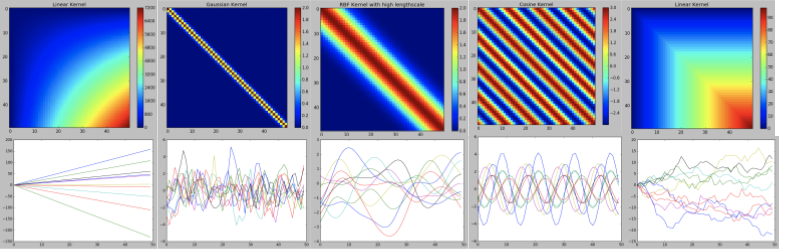
\includegraphics[scale=0.5]{thesis/images/Kernels_samples.png}
    \caption{Different Kernels and corresponding sampled GPs}
    \label{fig:generic_function_space}
\end{figure}

A covariance function, thus has two important responsibilities. First, when applied pairwise to the elements of set X it must be able to generate a proper covariance matrix (symmetric, positive semi definite etc.) and second, it should also somehow be a measure of nearness between two values, i.e. map its inputs to a real value. Former enables covariance function to significantly determine the properties of to be generated functions like smoothness, length-scale etc. from the corresponding GP to a large extent while latter means they are same as kernels of SVM literature [Kernel methods book ]

A Gaussian process is completely determined by its mean and co-variance function and once these two are fixed we can generate sample functions using equation \ref{eqn:GP_definition}  Fig 2.1: differnet covariance matrices and corresponding functions :  Shows A number of kernels and functions generated form corresponding  zero mean GPs. 

The mathematical literature on Gaussian process is quite extensive. [M Seeger’s paper and stochastic process book] are good references for detailed mathematical properties of GPs and of stochastic processes in general. [Bob 53, Grimment and Strizaker 1982> from OHagan book] are good references for application of GP in probability theory.

\subsubsection{Inference in GP}
Under Bayesian nonparametric framework, Gaussian processes are used to express our prior beliefs about underlying function that could describe observed data. By combining these prior assumptions with the observed information we arrive at the posterior representation of the latent function values.

A generic inference process of Gaussian process model which has n, Y ($[y_1,y_2,…y_n]$) values at locations X ($[x_1,x_2...x_n ]$) follows a hierarchical structure [Phd thesis RIhimaki]. 
First, we assume a data generating function $f_i = f(x_i)$ with n latent function values $f_1,f_2…f_n$ such that given these, Y’s are independent of locations X.
$$P(Y \mid F) = \Prod_{i=1}^{N}P(y_i \mid f_i)$$
The functional space from which these function values can arise is then constrained by putting a suitable GP prior over latent function values. $$ P(F(X) \mid \theta) = GP(m(X),K(X,X’ \mid \theta))$$
Finally, we can also put a prior over hyperparameters of covariance function, theta. 
	$$\theta ~ P(\theta)$$ 
Now, as explained in the section 2.2.2 a GP prior corresponds to a multivariate Gaussian distribution and hence prior for F can be written as:
$$P(F \mid X,\theta) = \mathbb{N}(F \mid 0, K_{xx})$$
Where $K_{xx}$ would be the covariance matrix generated through pairwise application of covariance function on observations X. Now following Bayesian inference rules the posterior can be obtained as,
\begin{equation}
P(F \mid X,Y,\theta) = \frac{P(Y \mid F)P(F \mid X, \theta)}{P(Y \mid X, \theta)} \approx \mathbb{N}(F \mid 0, K_{xx}) \prod_{i=1}^{n}P(y_i \mid f_i)
\label{eqn:GP_posterior}
\end{equation}

\subsubsection{Prediction}
Generally, we are also interested in the prediction of new latent values f* (or a new value y*) on different locations x*. In that case joint distribution of f and f* can be written as,
$$P(f,f^* \mid X,X*,y) ~ N([f, f*] | 0, [[K_{xx} K_{x*}],[K_{*x} K_{**}]])$$

Here $K_{x*}$ and $K_{**}$ are once again generated through pairwise application of covariance function on observed as well as new values and on new values respectively. $K_{x*}$ defines the covariance between new and observed function values while $K_{**}$ defines the covariance among new values.

Following conditional properties of Gaussian distribution [Bishop book, 87] we can generate distribution for f* given f as:
\begin{equation}
    P(f^* \mid f, X, x*) \approx \mathbb{N}(f^* \mid K_{*x}K_{xx}^{-1}f, K_{**} - K_{*x}K_{xx}^{-1}K_{x*} )
    \label{eqn:GP_prediction}
\end{equation}	 

Finally, if we are interested only in corresponding predicted values Y* it can be figured out as:
\begin{equation}
    P(y^* \mid Y, X, x*) \approx \Int P(y^* \mid f^*)P(f^* \mid X^*,Y,X)
\end{equation}
Here, $P(f^* \mid X^*,Y,X)$ is the posterior predictive distribution that can be obtained by integrating out the latent function values f from equation \ref{eqn:GP_prediction}

\subsubsection{Hyperparameter selection}

GP specifies a fully probabilistic model and hence it has a distinct advantage over other techniques that hyperparameters can be inferred from training data directly instead of using a cross validation scheme as in case of other methods. [luttinen’s thesis]
In a pure Bayesian framework, hyper-parameters would have priors set over them. However, complex relationship of hyper-parameters with covariance function means usually the integrals become intractable and must be done through other numerical methods like MCMC [W and R 2006] or likelihood maximization. Due to computational expensiveness of MCMC likelihood maximization is generally used for hyperparameter selection in GP. aA gradient based optimization procedure can be used thourgh Marginal data likelihood in the denominator of equation \ref{eqn:GP_posterior} to optimize hyperparameters,
$$P(Y \mid X, \theta) = \int P(Y \mid F)P(F \mid X, \theta) dF $$

Since the prior $P(F \mid X, \theta)$ is Gaussian ($\mathbb{N}(F \mid 0,K_{xx})$), after combining this with the Gaussian likelihood $P(Y \mid F) = \mathbb{N}(Y \mid F, \sigma^2)$ and integrating out F, the log marginal likelihood can be written as,

\begin{equation}
   log P(Y \mid X, \theta) = -\frac{1}{2}Y^{T}(K + \sigma^{2}I)^{-1}Y -\frac{1}{2} log (K + \sigma^{2}I) - \frac{n}{2} log \Pi
   \label{eqn:GP_likl}
\end{equation}

In the equation \ref{eqn:GP_likl} all the terms are a function of $\theta$. (K is calculated by pair wise application of function $k(\theta)$ on X) and hence optimal values of hyperparameters can be obtained by finding the gradient of  \ref{eqn:GP_likl} with respect to each $\theta_j \in \theta$

ML estimates might overfit sometimes however, a well peaked posterior drasitcally reduces overfitting risk of hyperparameters [Mackay 99]. 

\subsubsection{Regression using GP}
Gaussian process based Bayesian non parametric regression have been described in [Blight &Ott, hagan 1978, Neal 92] etc. The central idea is to first start with the parametric linear model and then generalize it through Gaussian processes. [W & R book] generalized regression by first using basis function to project standard linear regression to a high dimensional space and then using kernel trick [Kernel Methods book] to arrive at the same result as us section 2.2.3, this approach is also called the weight space view of Gaussian processes, details of which can be found in [oHagan 78, R & W book/paper , M Seeger]. 
Here we take a simpler approach based on the development of previous sections. Same equations can be arrived at using weight space view as illustrated in [http://dl.acm.org/citation.cfm?id=299093]
A generic regression problem can be defined as:
\begin{equation}
Y = f(x) + \epsilon(noise)
\label{eqn:regression}
\end{equation}
Where the objective is to find a good enough estimate of f(x) so that one could predict $Y^*$ values for input $X^*$. 
Traditional solution of the problem have been to use a parametric model similar to:
	$$F(x|w) = w_1 + w_2x + w_3x^2$$
Here w’s are also called the weights of the covariates. In Bayesian setting, w’s will be called the parameters and we put a prior p(w) on them. Once posterior $p(W \mid Y)$ is obtained we can predict new values using $p(Y^* \mid X^*, W)$. It can be observed that this approach quickly creates the problem of limiting the function capacity as explained in section 2.1. Moreover, it might also be difficult to encode prior beliefs about weights as a distribution p(W).

To provide an overly accommodating non linear functional space as prior for the desired regression function, we can put a Gaussian process prior over the weights. As explained in section 2.2 using GPs also alleviate the problem of providing our prior beliefs about parameters through covariance function and Kernels.

Thus the GP solution for regression problem in equation \ref{eqn:regression} becomes:

Prior: $P(f|X) = N(f| 0, K_{xx})$

where $K_xx$ is the covariance matrix for input X. 

We further assume Gaussian distribution for noise term in equation \ref{eqn:regression}:
	$$ \epsilon = N(0, \Sigma)$$
where $\Sigma = \sigma^2I$
Now following \ref{eqn:regression} likelihood of the observations is given by,

	$$ P(Y \mid F, X) = \mathbb{N}(f, \Sigma)$$

From here we can find the posterior in the similar way as in the section 2.3.2:
	
$$ P(f \mid X, Y) \approx \mathcal{N}(\mu_f, \S_f)$$

Here $\mu_f = (K_{xx}^{-1} + \Sigma^{-1})^{-1}\Sigma^{-1}Y$ and $S_f = (K_{xx}^{-1} + \Sigma^{-1})^{-1}$

Similarly, as in section Posterior predictive distribution for a new function value f* at point x* can be directly calculated using equation \ref{eqn:GP_prediction}

Regression is one of the simplest of Gaussian process use cases. [M seeger] provides pointers on to further generalize the model by allowing an arbitrary noise distribution directly in GP prior or extending it for other generalized linear models.  

\subsubsection{Classification using GP}
Classification is another common problem in machine learning in which desired functional value is categorical. In a generic classification setting, our observations include class labels Y ~ [1,2…M] corresponding to each data point X and our objective is to estimate a function F: X -> [1,2…M] that can assign the class labels appropriately to the new data points X* or in bayesian context finding the probability $P(y^* = c \mid x*, Y,X)$ where $c \in [1,2…M]$ 
The simplest case of GP classifier is called Bayesian discriminator [Ramsuseen Book, Barber and Williams] in which we consider a GP prior over the latent function and then the latent function values for data point are turned into class probabilities using a response function. This conversion of latent values of domain (–inf,+inf) to output of response function of domain (0,1) guarantees a valid probabilistic interpretation of our prediction. 
A common method to map the function values to probabilties is to use the logit function such that if y ~ {-1,1}  and $F_i$ is the latent function values for $X_i$:
	$$P(y_i \mid F_i)  = \sigma(y_i,f_i) = \frac{1}{(1+ exp^(-f_i))}$$

 Since the class labels are independent  from each other given latent function values, likelihood can be written as:
	$$ P(Y \mid F) = \Prod_(i=1)^{N} P(y_i \mid F_i) = \Prod_(i=1)^{N} \sigma(y_i,F_i)$$
	
Once again we put a GP prior on the latent function values $P(F \mid X) = \mathcal{GP}(F \mid \mu, K_{xx})$ and write the posterior as:
\begin{equation}
P(F \mid Y,X) = \frac{P(Y|F)P(F|X)}{P(Y \mid X)} = \frac{\mathcal{N}(F \mid 0, K_{xx})}{P(Y \mid X)}\Prod_{i=1}^{N}\sigma(y_i,F_i)
\end{equation}

Similarly, posterior predictive distribution of latent function is,
\begin{equation}
	P(F^* \mid X^*, Y,X) = \Int P(F^* \mid X^*, F ,X) p(F \mid X,Y) dF^*
\end{equation} 

Here $P(F^* \mid X^*, F ,X)$ is Gaussian that can be obtained through conditional GPs however, due to P(Y|F) and P(Y|X) being non Gaussian, both posterior and posterior predictive distribution become analytically intractable.
Since categorical predictions $y^*$ are much more important in classification context and we can still proceed for y* since we can integrate out the latent function values, 
$$P(y^*=+1 \mid X,Y,X^*) = \Int P(y* \mid F^*)P(F* \mid X,Y,X^*)dF^*$$

However, same as in previous case the integration is intractable and we must resort to approximation to obtain the distribution details. Section 2.3 describes variational inference scheme to find an approximation in the cases like this where an analytical  solution can not be obtained.
Apart from variational inference scheme described in next chapters, numerous other approximation solutions have been developed in for GP classification. An extensive survey of different approximation schemes for Classification using GPs can be found in  [http://mlg.eng.cam.ac.uk/pub/pdf/KusRas06.pdf] MOreover, Detailed treatment of more general cases of classification like multi-class classification or one class classification can be found in [Barber] and [http://hera.inf-cv.uni-jena.de:6680/pdf/Kemmler10:OCC.pdf] respectively.







\subsection{Approximate Inference in GP}[WIP]

\subsubsection{Approximate Inference}

In most of the cases, the solution of a Bayesian inference problem comes down to computing a posterior and a predictive posterior[BDA]. As we saw in section 2.2.5, calculating marginal data likelihood can also be significantly important for model selection and hyper-parameter optimization. 
As explained in the first section, if X is the data and z the parameter that govern it.
Computing posterior $p(Z|x)  = \frac{p(x|z)p(z)}{p(X)}$ where p(X) is the data likelihood and can be obtained as $p(X) = Int p(x|z)p(z)dz$. Finally prediction on a new data point $x^*$ can be obtained as
 	$$P(x^*|z) = Int p(x^*|z)p(z|x)dz$$		

Unfortunately, in most of practical considerations like GP classification (section 2.2.7) for example integrals mentioned in inference equations above become intractable. Traditionally, MMarkov Chain Monte Carlo (MCMC) methods - part of the generic stochastic family of approximations [Bishop’s book], have been employed to achieve the full integration results in the Bayesian problems for example, [http://omega.albany.edu:8008/neal.pdf], candidate method (Chib, 1995; and see Neal, 1998), bridge sampling and path sampling (Gelman and Meng, 1998) and the closely related Annealed Importance Sampling (Neal, 2001)] etc.
These techniques try to approximate the distribution by generating number of samples. Though MCMC guarantees to converge to the target distribution in the long run [http://www.cs.princeton.edu/courses/archive/spr06/cos598C/papers/AndrieuFreitasDoucetJordan2003.pdf: Jordan03], typically an extremely large number of samples is required to converge to accurate results.  Despite numerous advances in trying to make MCMC methods faster and efficient most of them still remain computationally prohibitive for most of the relevant models[ref?]. An extensive coverage of these stochastic techniques and their properties can be found in [BDA], similarly [Jordan 03] is a comprehensive introduction on MCMC applications from machine learning perspective. 

A number of other methods called deterministic methods [Bishop06, Minka thesis] approach the same task by trying to approximate posterior distribution using analytical approximations. These include Maximum likelihood and maximum a posteriori methods which approximate entire distribution to corresponding single point estimates [Murphy , Bishop book], thereby discarding all the uncertainties information associated with it. Laplace’s method, on the other hand, approximates true distribution by a Gaussian distribution that matches the mode, first derivative and second derivative of the former [Mackay’s book]. Another family of methods include Expectation propagation [Minka’s 01 ] and Variational Bayes [Jordan et al. 98] that try to obtain a simpler distribution closest to the target distribution based on information theoretic distance metrics like KL divergence.  
Compared to MCMC methods, deterministic methods generally aren’t able to recover the target distribution exactly. However their computational efficiency and versatility makes them a very useful method in approximate inference toolbox. In the following section we describe variational bayes in more detail.

\subsubsection{Variational Inference}[WIP]


\subsubsection{Variational Infernece in GP }[WIP]

\subsubsection{Sparse approximaiton in GP [WIP]}
%%\subsection{Gaussian Processes}
Due to their seemingly simple nature and interesting analytical properties Gaussian processes have been used extensively in various tasks for centuries. Flexibility of Gaussian Processes have seen them employed in various forms. [BDA reference about 1800 century], Gelmen et al. mention them being used for astronomical data modelling in 18th century. Later, significant work have been done as part of stochastic process literature for example as Weiner processes and later for time series prediction[Weiner process, A Populi’91 reference for stochastic process and other Reference from Phd thesis]. In Spatial statistics, gaussian process regression was used for interpolation of values based on space as the input by Matheron in 1973 following the work of D.G. Krige [ both references from wiki]. In applied statistics context, Gaussian processes were first used for regression and classification [O’Hagan 1978], density estimation [reference from BDA, rihimaki thesis and other one ] etc. Inspired by the link shown between neural networks and Gaussian process by [Neal ‘ 96] Gaussian processes were quickly extended to machine learning context[Rasmussen 96]. With the advent of approximation schemes [Sparse approximation referneces] and hardware gains, use of Gaussian process has quickly skyrocketed in other areas of machine learning such as dimensionality reduction [reference], latent vector modelling [reference], even multi purpose deep Gaussian processes analogous to deep neural network have been proposed [GPRN paper, deep GP paper].  In the next few sections, we first define Gaussian processes and review it's properties like covariance functions etc briefly and later describe the inference procedure including  predictions and parameter selection in Section 2.2 
\subsubsection{Definition}
A function is generally thought of as a mapping from an arbitrary set X to another F(X), $X -> F(X)$. One interesting way to look at it can be of thinking X and F(X) as infinitely long vectors with former’s elements acting as an index for the latter, i.e. X as an index set for F(X).  A collection of these random mappings is called a process [Random Fields and geometry, Andler, Stochastic process book]. 

A Gaussian Process is thus formally defined as a collection of random variables, any finite set of which is jointly distributed. i.e. for a finite set x contained in X , collection of random variables F(x) will follow a Gaussian distribution [GPML book], i.e. 

\begin{equation}
    p(F|X) ~ mathbb{N}(m,K)
    \label{eqn:GP_definition}
\end{equation} 

In gaussian process terms f(x) is written as $f(x) ~ GP(m(x),k(x,x))$ where m(x) and k(x,x) are called the mean and covariance function respectively. 

\subsubsection{Covariance functions and Kernels}

From a function perspective, one expects that data points close/near to each other will have similar values. This notion of nearness can also be seen in general life for example, if one were to measure moisture in environment at a specific time every day for a year we expect days or places near each other to have similar temperatures. Gaussian Process represent this concept of nearness/closeness through a covariance function, i.e. how the function value changes with respect to the difference in their index values. Thus, a covariance function must take two indices and map them to a real number defining the correlation of underlying function’s values at the indices. 
The matrix K in equation \ref{eqn:GP_definition} is generated by applying this covariance function for each pair of elements in X. 
\begin{figure}
    \centering
    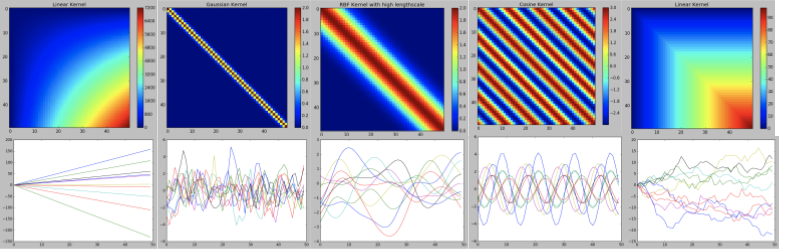
\includegraphics[scale=0.5]{thesis/images/Kernels_samples.png}
    \caption{Different Kernels and corresponding sampled GPs}
    \label{fig:generic_function_space}
\end{figure}

A covariance function, thus has two important responsibilities. First, when applied pairwise to the elements of set X it must be able to generate a proper covariance matrix (symmetric, positive semi definite etc.) and second, it should also somehow be a measure of nearness between two values, i.e. map its inputs to a real value. Former enables covariance function to significantly determine the properties of to be generated functions like smoothness, length-scale etc. from the corresponding GP to a large extent while latter means they are same as kernels of SVM literature [Kernel methods book ]

A Gaussian process is completely determined by its mean and co-variance function and once these two are fixed we can generate sample functions using equation \ref{eqn:GP_definition}  Fig 2.1: differnet covariance matrices and corresponding functions :  Shows A number of kernels and functions generated form corresponding  zero mean GPs. 

The mathematical literature on Gaussian process is quite extensive. [M Seeger’s paper and stochastic process book] are good references for detailed mathematical properties of GPs and of stochastic processes in general. [Bob 53, Grimment and Strizaker 1982> from OHagan book] are good references for application of GP in probability theory.

\subsubsection{Inference in GP}
Under Bayesian nonparametric framework, Gaussian processes are used to express our prior beliefs about underlying function that could describe observed data. By combining these prior assumptions with the observed information we arrive at the posterior representation of the latent function values.

A generic inference process of Gaussian process model which has n, Y ($[y_1,y_2,…y_n]$) values at locations X ($[x_1,x_2...x_n ]$) follows a hierarchical structure [Phd thesis RIhimaki]. 
First, we assume a data generating function $f_i = f(x_i)$ with n latent function values $f_1,f_2…f_n$ such that given these, Y’s are independent of locations X.
$$P(Y \mid F) = \Prod_{i=1}^{N}P(y_i \mid f_i)$$
The functional space from which these function values can arise is then constrained by putting a suitable GP prior over latent function values. $$ P(F(X) \mid \theta) = GP(m(X),K(X,X’ \mid \theta))$$
Finally, we can also put a prior over hyperparameters of covariance function, theta. 
	$$\theta ~ P(\theta)$$ 
Now, as explained in the section 2.2.2 a GP prior corresponds to a multivariate Gaussian distribution and hence prior for F can be written as:
$$P(F \mid X,\theta) = \mathbb{N}(F \mid 0, K_{xx})$$
Where $K_{xx}$ would be the covariance matrix generated through pairwise application of covariance function on observations X. Now following Bayesian inference rules the posterior can be obtained as,
\begin{equation}
P(F \mid X,Y,\theta) = \frac{P(Y \mid F)P(F \mid X, \theta)}{P(Y \mid X, \theta)} \approx \mathbb{N}(F \mid 0, K_{xx}) \prod_{i=1}^{n}P(y_i \mid f_i)
\label{eqn:GP_posterior}
\end{equation}

\subsubsection{Prediction}
Generally, we are also interested in the prediction of new latent values f* (or a new value y*) on different locations x*. In that case joint distribution of f and f* can be written as,
$$P(f,f^* \mid X,X*,y) ~ N([f, f*] | 0, [[K_{xx} K_{x*}],[K_{*x} K_{**}]])$$

Here $K_{x*}$ and $K_{**}$ are once again generated through pairwise application of covariance function on observed as well as new values and on new values respectively. $K_{x*}$ defines the covariance between new and observed function values while $K_{**}$ defines the covariance among new values.

Following conditional properties of Gaussian distribution [Bishop book, 87] we can generate distribution for f* given f as:
\begin{equation}
    P(f^* \mid f, X, x*) \approx \mathbb{N}(f^* \mid K_{*x}K_{xx}^{-1}f, K_{**} - K_{*x}K_{xx}^{-1}K_{x*} )
    \label{eqn:GP_prediction}
\end{equation}	 

Finally, if we are interested only in corresponding predicted values Y* it can be figured out as:
\begin{equation}
    P(y^* \mid Y, X, x*) \approx \Int P(y^* \mid f^*)P(f^* \mid X^*,Y,X)
\end{equation}
Here, $P(f^* \mid X^*,Y,X)$ is the posterior predictive distribution that can be obtained by integrating out the latent function values f from equation \ref{eqn:GP_prediction}

\subsubsection{Hyperparameter selection}

GP specifies a fully probabilistic model and hence it has a distinct advantage over other techniques that hyperparameters can be inferred from training data directly instead of using a cross validation scheme as in case of other methods. [luttinen’s thesis]
In a pure Bayesian framework, hyper-parameters would have priors set over them. However, complex relationship of hyper-parameters with covariance function means usually the integrals become intractable and must be done through other numerical methods like MCMC [W and R 2006] or likelihood maximization. Due to computational expensiveness of MCMC likelihood maximization is generally used for hyperparameter selection in GP. aA gradient based optimization procedure can be used thourgh Marginal data likelihood in the denominator of equation \ref{eqn:GP_posterior} to optimize hyperparameters,
$$P(Y \mid X, \theta) = \int P(Y \mid F)P(F \mid X, \theta) dF $$

Since the prior $P(F \mid X, \theta)$ is Gaussian ($\mathbb{N}(F \mid 0,K_{xx})$), after combining this with the Gaussian likelihood $P(Y \mid F) = \mathbb{N}(Y \mid F, \sigma^2)$ and integrating out F, the log marginal likelihood can be written as,

\begin{equation}
   log P(Y \mid X, \theta) = -\frac{1}{2}Y^{T}(K + \sigma^{2}I)^{-1}Y -\frac{1}{2} log (K + \sigma^{2}I) - \frac{n}{2} log \Pi
   \label{eqn:GP_likl}
\end{equation}

In the equation \ref{eqn:GP_likl} all the terms are a function of $\theta$. (K is calculated by pair wise application of function $k(\theta)$ on X) and hence optimal values of hyperparameters can be obtained by finding the gradient of  \ref{eqn:GP_likl} with respect to each $\theta_j \in \theta$

ML estimates might overfit sometimes however, a well peaked posterior drasitcally reduces overfitting risk of hyperparameters [Mackay 99]. 

\subsubsection{Regression using GP}
Gaussian process based Bayesian non parametric regression have been described in [Blight &Ott, hagan 1978, Neal 92] etc. The central idea is to first start with the parametric linear model and then generalize it through Gaussian processes. [W & R book] generalized regression by first using basis function to project standard linear regression to a high dimensional space and then using kernel trick [Kernel Methods book] to arrive at the same result as us section 2.2.3, this approach is also called the weight space view of Gaussian processes, details of which can be found in [oHagan 78, R & W book/paper , M Seeger]. 
Here we take a simpler approach based on the development of previous sections. Same equations can be arrived at using weight space view as illustrated in [http://dl.acm.org/citation.cfm?id=299093]
A generic regression problem can be defined as:
\begin{equation}
Y = f(x) + \epsilon(noise)
\label{eqn:regression}
\end{equation}
Where the objective is to find a good enough estimate of f(x) so that one could predict $Y^*$ values for input $X^*$. 
Traditional solution of the problem have been to use a parametric model similar to:
	$$F(x|w) = w_1 + w_2x + w_3x^2$$
Here w’s are also called the weights of the covariates. In Bayesian setting, w’s will be called the parameters and we put a prior p(w) on them. Once posterior $p(W \mid Y)$ is obtained we can predict new values using $p(Y^* \mid X^*, W)$. It can be observed that this approach quickly creates the problem of limiting the function capacity as explained in section 2.1. Moreover, it might also be difficult to encode prior beliefs about weights as a distribution p(W).

To provide an overly accommodating non linear functional space as prior for the desired regression function, we can put a Gaussian process prior over the weights. As explained in section 2.2 using GPs also alleviate the problem of providing our prior beliefs about parameters through covariance function and Kernels.

Thus the GP solution for regression problem in equation \ref{eqn:regression} becomes:

Prior: $P(f|X) = N(f| 0, K_{xx})$

where $K_xx$ is the covariance matrix for input X. 

We further assume Gaussian distribution for noise term in equation \ref{eqn:regression}:
	$$ \epsilon = N(0, \Sigma)$$
where $\Sigma = \sigma^2I$
Now following \ref{eqn:regression} likelihood of the observations is given by,

	$$ P(Y \mid F, X) = \mathbb{N}(f, \Sigma)$$

From here we can find the posterior in the similar way as in the section 2.3.2:
	
$$ P(f \mid X, Y) \approx \mathcal{N}(\mu_f, \S_f)$$

Here $\mu_f = (K_{xx}^{-1} + \Sigma^{-1})^{-1}\Sigma^{-1}Y$ and $S_f = (K_{xx}^{-1} + \Sigma^{-1})^{-1}$

Similarly, as in section Posterior predictive distribution for a new function value f* at point x* can be directly calculated using equation \ref{eqn:GP_prediction}

Regression is one of the simplest of Gaussian process use cases. [M seeger] provides pointers on to further generalize the model by allowing an arbitrary noise distribution directly in GP prior or extending it for other generalized linear models.  

\subsubsection{Classification using GP}
Classification is another common problem in machine learning in which desired functional value is categorical. In a generic classification setting, our observations include class labels Y ~ [1,2…M] corresponding to each data point X and our objective is to estimate a function F: X -> [1,2…M] that can assign the class labels appropriately to the new data points X* or in bayesian context finding the probability $P(y^* = c \mid x*, Y,X)$ where $c \in [1,2…M]$ 
The simplest case of GP classifier is called Bayesian discriminator [Ramsuseen Book, Barber and Williams] in which we consider a GP prior over the latent function and then the latent function values for data point are turned into class probabilities using a response function. This conversion of latent values of domain (–inf,+inf) to output of response function of domain (0,1) guarantees a valid probabilistic interpretation of our prediction. 
A common method to map the function values to probabilties is to use the logit function such that if y ~ {-1,1}  and $F_i$ is the latent function values for $X_i$:
	$$P(y_i \mid F_i)  = \sigma(y_i,f_i) = \frac{1}{(1+ exp^(-f_i))}$$

 Since the class labels are independent  from each other given latent function values, likelihood can be written as:
	$$ P(Y \mid F) = \Prod_(i=1)^{N} P(y_i \mid F_i) = \Prod_(i=1)^{N} \sigma(y_i,F_i)$$
	
Once again we put a GP prior on the latent function values $P(F \mid X) = \mathcal{GP}(F \mid \mu, K_{xx})$ and write the posterior as:
\begin{equation}
P(F \mid Y,X) = \frac{P(Y|F)P(F|X)}{P(Y \mid X)} = \frac{\mathcal{N}(F \mid 0, K_{xx})}{P(Y \mid X)}\Prod_{i=1}^{N}\sigma(y_i,F_i)
\end{equation}

Similarly, posterior predictive distribution of latent function is,
\begin{equation}
	P(F^* \mid X^*, Y,X) = \Int P(F^* \mid X^*, F ,X) p(F \mid X,Y) dF^*
\end{equation} 

Here $P(F^* \mid X^*, F ,X)$ is Gaussian that can be obtained through conditional GPs however, due to P(Y|F) and P(Y|X) being non Gaussian, both posterior and posterior predictive distribution become analytically intractable.
Since categorical predictions $y^*$ are much more important in classification context and we can still proceed for y* since we can integrate out the latent function values, 
$$P(y^*=+1 \mid X,Y,X^*) = \Int P(y* \mid F^*)P(F* \mid X,Y,X^*)dF^*$$

However, same as in previous case the integration is intractable and we must resort to approximation to obtain the distribution details. Section 2.3 describes variational inference scheme to find an approximation in the cases like this where an analytical  solution can not be obtained.
Apart from variational inference scheme described in next chapters, numerous other approximation solutions have been developed in for GP classification. An extensive survey of different approximation schemes for Classification using GPs can be found in  [http://mlg.eng.cam.ac.uk/pub/pdf/KusRas06.pdf] MOreover, Detailed treatment of more general cases of classification like multi-class classification or one class classification can be found in [Barber] and [http://hera.inf-cv.uni-jena.de:6680/pdf/Kemmler10:OCC.pdf] respectively.








%% In a thesis, every section starts a new page, hence \clearpage

%% In a thesis, every section starts a new page, hence \clearpage
\clearpage
\section{Latent Variable Models}

\thispagestyle{empty}
Latent variable models have been a cornerstone of complex, high dimensional data analysis for a long time. They are slightly different from the methods mentioned earlier in the sense that here one tries to understand the underlying data structure by assuming that the observations are a result of interaction between an unknown number of hidden or latent variables (Raiko et al., 2006) and hence the objective is to learn both the hidden variables and the interaction or process.

The latent representations learnt during data analysis can be very task specific for example, in order to reduce dimensionality these learned representations can summarise the most relevant aspects of high dimensional data in fewer dimensions or can aid in recognizing patterns by extracting important non measurable aspects or features from data. Thus latent variable models provide a simple flexible framework under which various different statistical methods can be unified (Bartholomew, Knott, & Moustaki, 2011).  

If we consider latent variable as the parameters of data, the idea of learning hidden variables and the process through which they generate observations closely follows the Bayesian inference process described in section 1 and inverse of generation process can also be referred as projection of data to latent space. This interaction between latent variables or mapping to latent space can be linear or non-linear. Linear interactions like FA, PCA, ICA [hyvornen et al?] etc, though interpretable due to their simplicity and computationally fast, may not be suitably in cases where a complex latent space mapping is to be found. Non linear interactions on the other hand can provide enough capacity to model complicated processes at the cost of interpretability and computational ease. Self organizing maps [Karhunen], non linear PCA[Valpola 2004], Gaussian process latent vector model [], non linear space mdoels [Valpola 2005] are some of the examples of non linear LVMs.

In the following subsections we first describe the foundational linear model called Factor Analysis froma probabilsitic perspective and then move on to a more sophisticated latent model called GP based FA. 

\subsection{Probabilistic Factor Analysis}
Originated from in psychological research in early 19th century, Factor models are considered one of the oldest linear latent variable methods (Bartholomew et al., 2011). It derives its name from two factor model presented by (Spearman, 1904) postulating that test scores of individuals can be thought of as linear combinations of two factors, namely common factor- akin to one’s general intelligence and another specific to the context of test (Anderson & Rubin, 1956). 

Central objective behind factor analysis is to describe the co-variance among large number of observed variables in terms of less number of underlying latent variables, called factors. This ability to explain away the variation can also enable factors to express commonalities hidden in data, making them very suitable tool for extrapolatory data analysis.

Consider an observed data set ${Y \in N \times P}$ and factors ${X \in N \times Q}$, where commonly ${Q << P}$. According to traditional FA model(Anderson & Rubin, 1956; Bartholomew et al., 2011), each instance of Y is assumed to be generated by a linear transformation of uncorrelated factors X such that , 
\begin{equation}
Y_i = \Phi X_i + \mu + E_i, 
\end{equation}

Where, ${\Phi}$ is a constant matrix representing the linear transformation of factors X. Values of ${\Phi}$ correspond the amount of influence a particular factor has on the observed data and thus are appropriately named as factor loadings, ${\mu}$ is the mean vector. Factors ${X_i}$ as well as noise ${E_i}$ are assumed to be Gaussian distributed as ${\mathcal{N}(X_i| 0, I)}$ and ${\mathcal{N}(E_i | 0,\Psi)}$ respectively. 

This gives us a normally distributed generative model of data given by,
\begin{equation}
Y_i \in \mathcal{N}(Y_i | \mu,  \Phi\Phi^T + \Psi)
\end{equation}

It can be observed that if ${\Psi}$ is a diagonal matrix estimated from observations, covariance in Y can be solely explained by the latent factors while ${E_i}$ models the individual variability of each data instance ${Y_i}$. A detailed review of various properties of FA models can be found in (Bartholomew et al., 2011).

Due to its popularity, a number of inference methods both Bayesian and non Bayesian have been proposed to estimate FA parameters over time (Anderson & Rubin, 1956; Jöreskog, 1967; Lawley, 1940; Press & Shigemasu, 1989; Rowe, Rowe, & Press, 1998; Rubin & Thayer, 1982). In addition to the ability of including prior or expert knowledge about factors, Bayesian approaches have added consequence of eliminating rotational ambiguity in estimation of factor loadings.

In Bayesian formulation of Factor analysis, we put a prior over factor loading matrix ${\Phi}$ and substitute error covariance matrix ${\Psi}$ with its inverse, precision matrix ${\psi}$.
\begin{equation}
p(\Phi) = \prod_{q=1}^{Q} \mathcal{N}(\phi_q | 0, f_q^{-1}I)
\end{equation}
\begin{equation}
p(f) = \prod_{q=1}^{Q} \mathcal{G}(f_q | a_{q}^{f}, a_{q}^{f})
\end{equation}
\begin{equation}
 p(\psi) =  \mathcal{G}(\psi | a^{\psi}, b^{\psi}) \hspace{1em}, \psi = \Psi^{-1}.
\end{equation}

Here, ${\phi_k}$ represents kth column of the loading matrix (or kth factor) which is isotropically Gaussian distributed with the precision matrix represented by ${f_k}$.Precision matrices ${\psi}$ and ${f_k}$ are given Gamma priors controlled by their respective hyper-parameters. Being the precision of zero mean Gaussian, ${f_k}$  can be used to shut off corresponding redundant factors.

Joint posterior distribution of parameters ${p(\Phi, X, \mu, \psi, f | Y )}$  is analytically intractable and must be approximated. (Ghahramani \& Beal, 2000; Nielsen, 2004) provide detailed derivations for variational inference over a fully factorized approximated distributions of this posterior. However, these methods are known to have some downsides like heavier penalization of model or inability of solution to shut down redundant factors specially in observations with minimal noise which was more recently overcome by (Zhao & Yu, 2009) in their improved VB schemes.

Distributional assumptions of factors and noise terms in FA are of utmost importance since slight variations in them result in a variety of different models with significantly different characteristics. Principal component analysis (Jolliffe, 2002), for example is considered a special case of FA in which noise is kept same for every factor (i.e. ${\Psi_k}$ = ${Psi}$). (Tipping \& Bishop, 1999) further showed that as ${\Psi}$ approaches infinity ML estimation of FA tends to approach in standard PCA results. Similarly, a non Gaussian assumption of the factors lead us to ICA model, enabling factors (or components) to be truly independent from each other. Introduction of fixed or time varying state dynamics within factors is called linear state space model, another extension of FA models (Luttinen, Raiko, & Ilin, 2014). 

All of these models are closely related to each other due to their linear Gaussian assumptions. A detailed review of latent linear Gaussian models can be found in (Roweis \& Ghahramani, 1999).

\subsection{GP based Factor analysis model}

One way to achieve temporal structures within factor models is by putting GP priors over the factors. This lets us specify the relationship between latent values of a factor with the help of covariance functions.

These methods are popular in scenarios where observations correspond to some varying phenomenon like time series [Neural paper] and/or locations [luttinen’s paper]. Moreover, GP based LVMs have also been used in a multiple response setting [Seeger] where GP were used to model the dependencies between response variables. These are called semi-parametric models due to them being a combination of Non-parametric properties of GP and parametric linear mixing of factors. 
The model we describe here is different from [Luttinen’s] in the sense that it parameterizes the mixing matrix $\Phi$ rather than making it non-parametric. [Seeger] proposes a very similar model in a multiple response setting and uses IVM framework [lawrence] for the posterior approximation that can be heafty with larger data sets. In next section we provide a VB based inference along with a sparse approximation that should be computationally efficient specially for larger data sets. Similarly, the distinction form [Neural] lies in it not being applicable only in time series data. 
\begin{wrapfigure}{l}{0.35\textwidth}
    \centering
    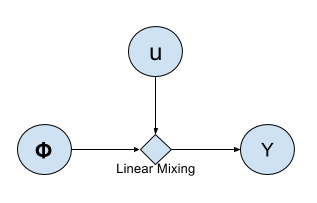
\includegraphics[scale=0.5]{images/GPFA_graphical_model.png}
    \caption{Graphical representation of GP based factor analysis model}
    \label{fig:gpfa_graph}
\end{wrapfigure}

Mathematically, model is very similar to the standard factor model described in previous section with the distinction that here latent factors $u$ are assumed to be conditionally independent GP, indexed through a common index $x$. As can be observed from Figure \ref{fig:gpfa_graph}, flow of information from each observed response to every latent factor response makes the sharing of statistical strength among response variables possible, thereby resulting in a much more expressive model than traditional factor analysis models. 
\newpage

The model is shown in figure \ref{fig:gpfa_graph} and can be expressed as,
\begin{equation}
Y=\phi u + \sigma^2I
\end{equation}

where ${u \in R^{P \times N}}$ are the latent factors that get linearly mixed through matrix  ${\phi \in R^{C \times P},}$ resulting in the observations ${Y \in R^{C \times N}}$. As in [Seeger], factor analysis emerges when $P << C $ 

We put a GP prior on latent variables $ u_p \in GP(0,K^p)$ where $K^p$ is the co-variance kernel for that particular Gaussian process. Loading matrix $\phi$ is assumed to have a Gaussian prior $N(0,I)$. 

\subsubsection{Variational Sparse Approximation of GPFA posterior}

To achieve sparsity in posterior, we approximate the posterior distribution as $ q(\phi,u,\hat{u})$ where  $p(\hat{u})$ is the distribution through n inducing points ( n << N). Finally, a GP prior is put on $p(\hat{u})$ too and the sparse approximation of posterior to factorizes as: 
\begin{equation}
q(\phi,u,\hat{u}) = q(\phi)\prod_{p=1}^{P}p(u_p \mid \hat{u_p})q(u_p)
\end{equation}

Based on above sparse approximation, marginal likelihood of data can be given as,
\begin{equation}
L(Y|X) = \int p(Y \mid \hat{u},\phi) p(\phi,\hat{u},u) d\phi du d\hat{u}
\label{eqn:gpfa_lklihd}
\end{equation}

Following the VB inference scheme as outlined in section 3, we find optimal distributions by minimizing the KL divergence between approximation and true posterior. This in turn is equivalent to maximizing the log of marginal likelihood given in equation \ref{eqn:gpfa_lklihd} with respect to each parameter(detailed derivations are given in Appendix 1) :

For $\hat{u_p}$, 
$${q(\hat{u}_p) \approx \mathcal{N}(\hat{u}_p \mid \Sigma_{p}^{-1}K_{nn}^{-1}K_{Nn}Z_p,\Sigma_{p}^{-1})
}$$
where, ${
\Sigma_{p} = K_{nn}^{-1} + \frac{1}{\sigma^2}K_{nn}^{-1}K_{nN}S_pK_{Nn}K_{nn}^{-1}}$ and 
${Z_p = \sum_{c}^{C}\mathbb{E}[\phi_{cp}](y_c - \sum_{i}^{P/p}\mathbb{E}[\phi_{ci}]\mathbb{E}[u_{ip}])}$.   

Similarly VB update for $\hat{\phi}$ can be derived as, 
$${q(\phi) \approx \mathcal{N}(\phi \mid y\mathbb{E}[U]^T\Sigma_{\phi}^{-1}, \Sigma_{\phi})}$$
where ${\Sigma_{\phi} = (V_{\phi}^{-1} + I )^{-1}}$
and ${V_{\phi} = \mathbb{E}[u]\mathbb{E}[u]^T\sigma^2}$

Finally update for ${u}$ is,
$${
q(u_p) \approx \mathcal{N}(u_p \mid M\hat{\mu_{p}}, \Sigma_{u \mid \hat{u}}^{p} + M\Sigma_pM^T)
}$$
where ${\hat{\mu_{p}}$ is the mean of GP $u_p$, ${M = K_{Nn}K_{nn}^{-1} }$ and
${\Sigma_{u\mid\hat{u}}^{p} = K_{NN} - MK_{nN} }$

\subsubsection{Hyper-parameter selection}
Hyperparameters for GP based FA that might require tuning mostly include the parameters for covariance kernel function of GPs corresponding to the latent factors. These can be optimized  by maximizing the marginal log likelihood with respect to the latent factors as:
\begin{equation}
L(\theta_p) = log \mathcal{N}(S_{p}^{-1}z_p \mid 0,S_{p}^{-1} + K_{Nn}K_{nn}^{-1}K_{nN}) - \frac{1}{2}tr(\sum_{i=1}^{P}S_{i}*cov(u_i \mid \hat{u}_i)) ) + consts.
\label{eqn:gpfa_likl_opt}
\end{equation}
where $S_p = \sum_{c}^{C}\mathbb{E}[\phi_{cp}^2]$

Using above equation one can obtain the gradients by differentiating the log likelihood corresponding to  each parameter $\theta_{p}$ of co-variance kernels associated with respective late factor GP. Recommended method of inference would be to first optimize hyperparameters and then find optimal distributions through VB updates while keeping the hyperparameters fixed. 

\subsubsection{Demonstrations on artificial data set}
\begin{figure}
    \centering
    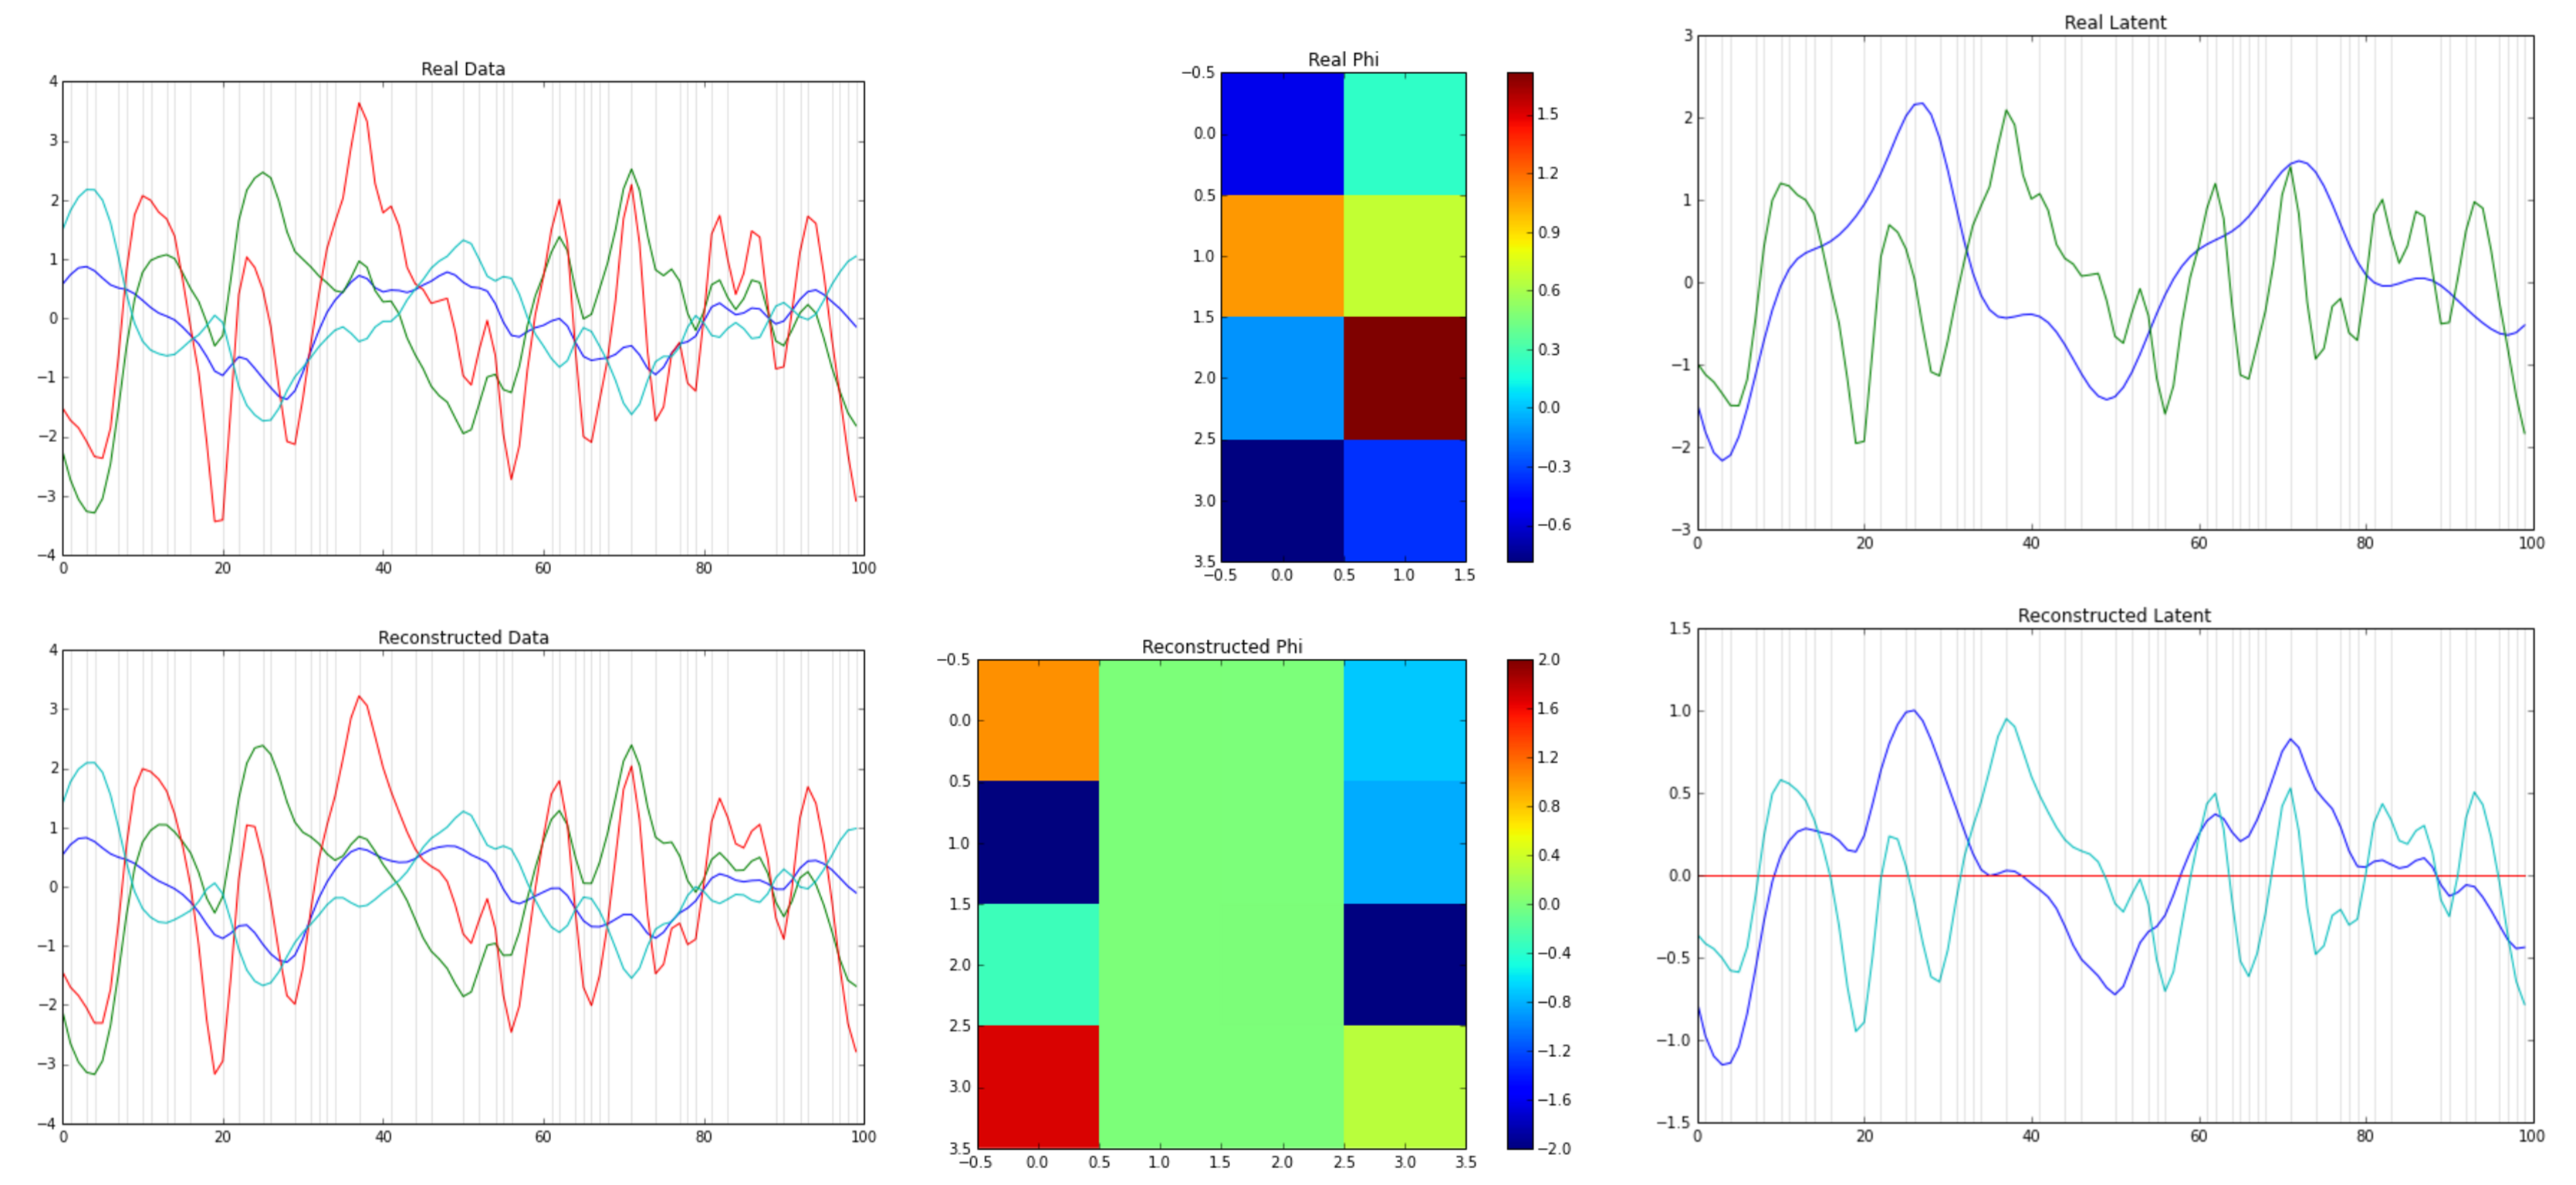
\includegraphics[scale=0.25]{thesis/images/SLFM_demo1.png}
    \caption{Extracting latent processes from artificial data set using GPFA: Upper row shows the real latent process and mixing matrix. Second row demonstrates the extracted latent structure using variational inference. Gray Spikes indicate the inducing points at which functions were evaluated}
    \label{fig:slfm_demo1}
\end{figure}

In order to demonstrate model’s ability to recover latent processes that might have been used in data generation processes, We generated two artificial data sets using distinct latent process sets. 

First data set was created by mixing two latent processes (using 100 evaluation points) with the squared exponential kernel and using a randomly generated mixing matrix. We then initialized the variational algorithm with four random latent processes with SE of lengthscale and variance one. The inducing set $u_p$ was chosen to be only half of the original data set selected randomly. As can be seen in the Figure \ref{fig:slfm_demo1} , the model was not only able to recover the latent process structure very well but also shut off two redundant latent processes acting very similar to ARD prior [Reference?]. Since the variational approximation recovers complete distribution of the latent processes as well as the loading matrix, it is possible to augment these values with the confidence (something that’s not possible in SLFM for mixing matrix).

\begin{figure}
    \centering
    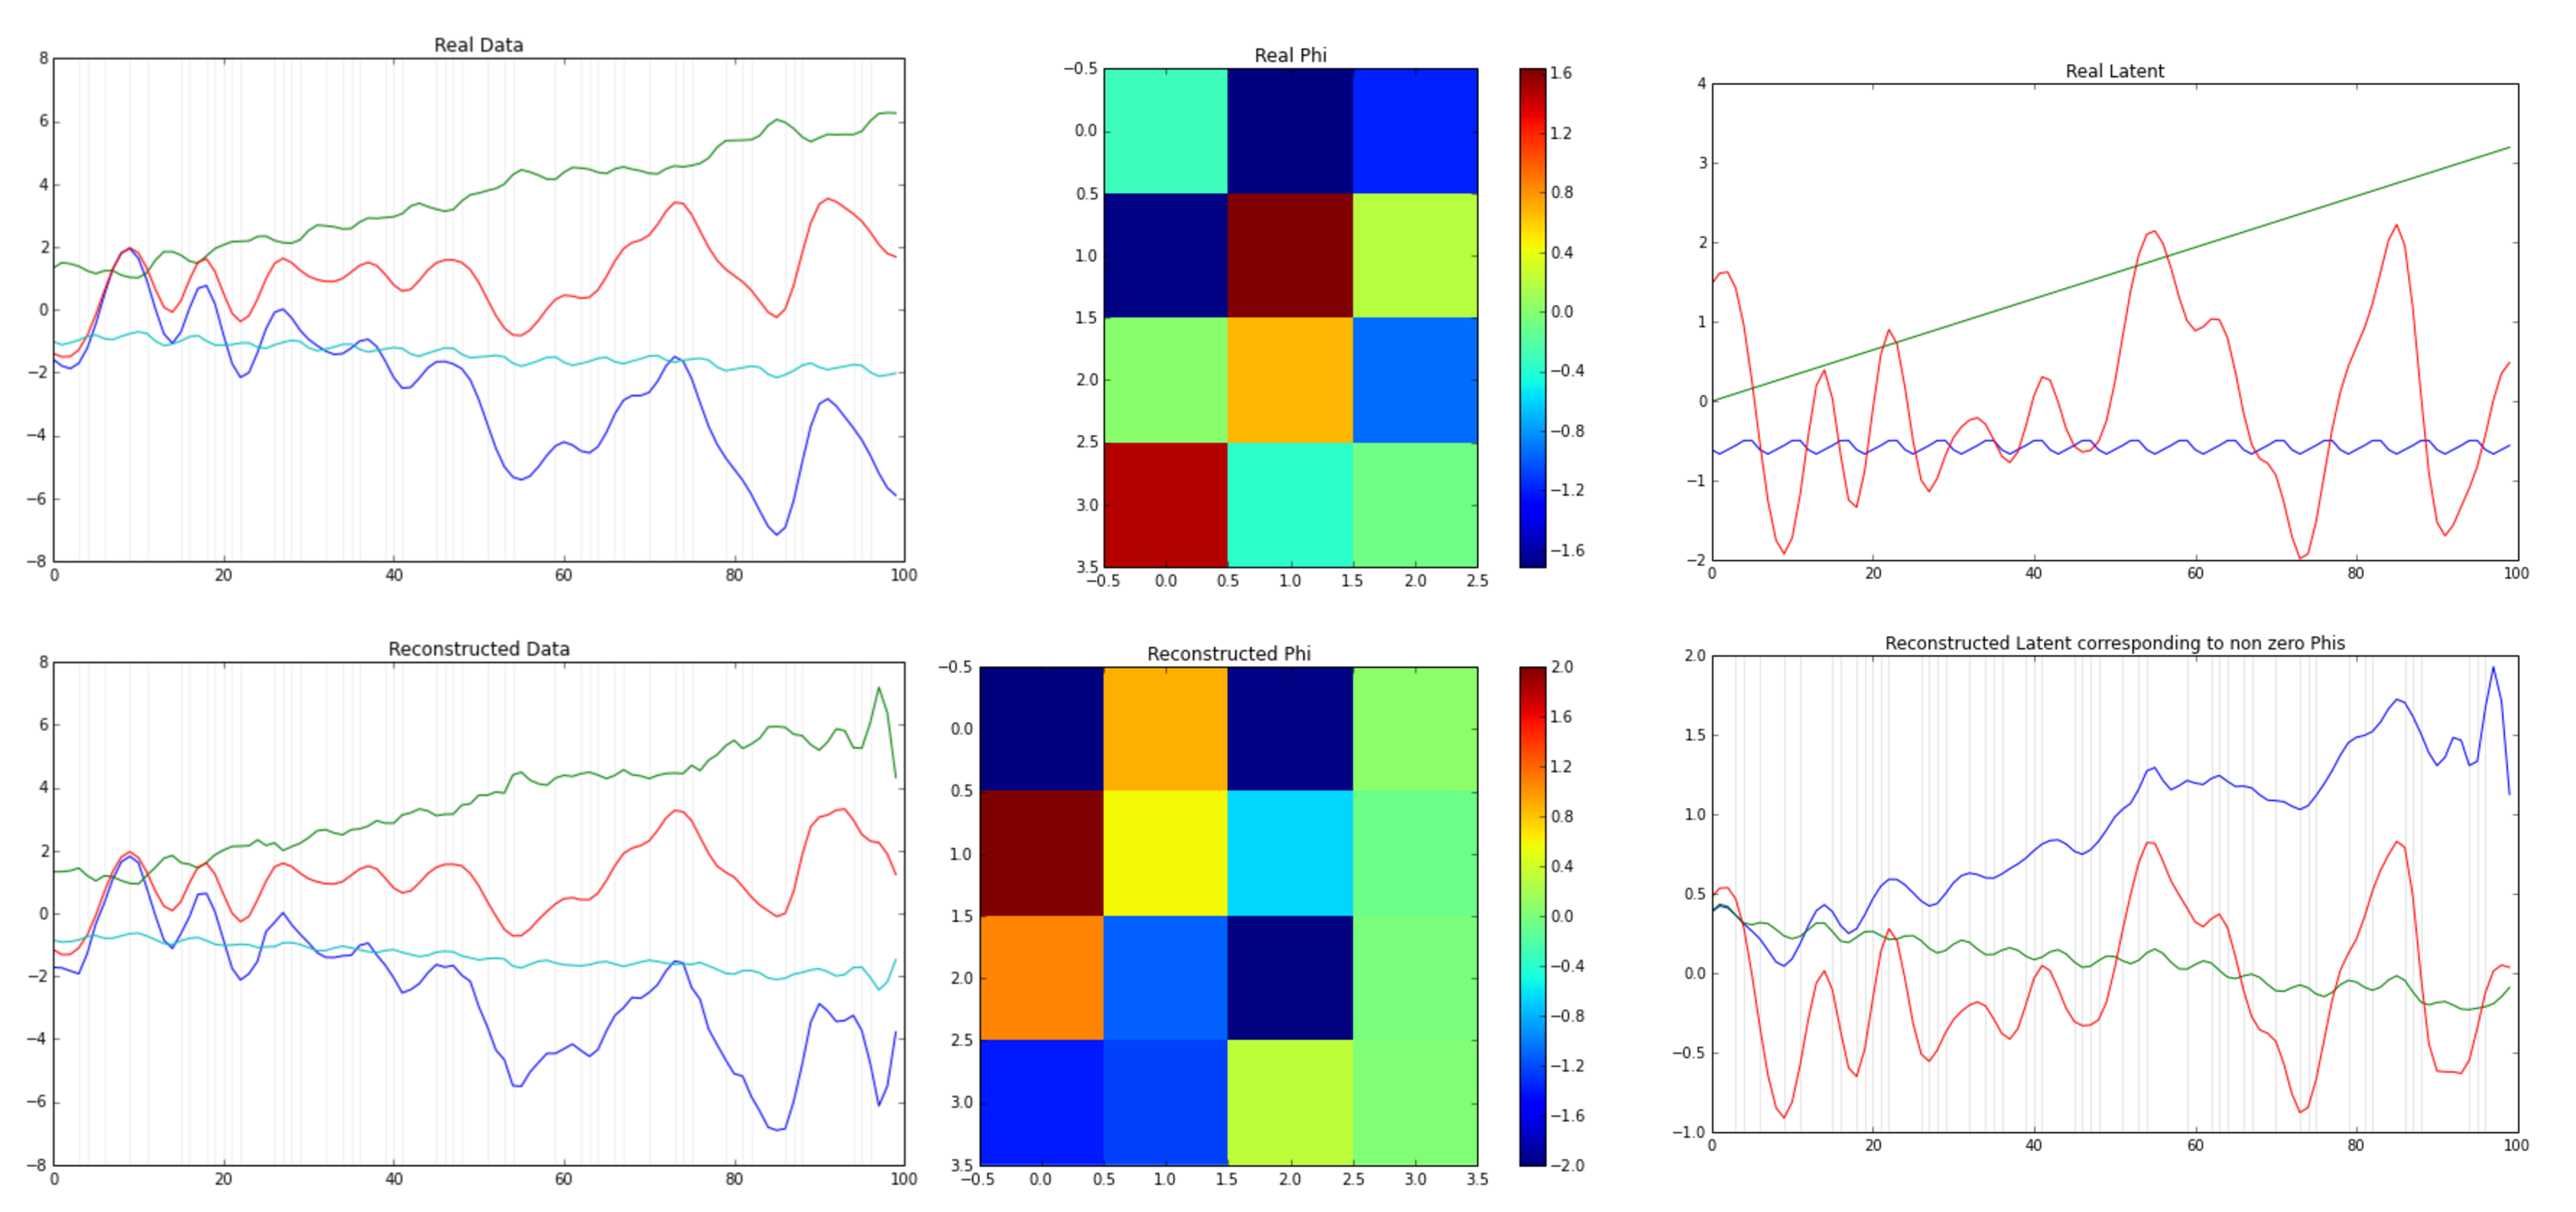
\includegraphics[scale=0.25]{thesis/images/SLFM_demo2.png}
    \caption{Extracting latent processes from artificial data set using GPFA: Upper row shows the real latent process (with periodic, linear and Gaussian kernels) and mixing matrix. Second row demonstrates the extracted latent structure using variational inference. Gray Spikes indicate the inducing points at which functions were evaluated}
    \label{fig:slfm_demo2}
\end{figure}

Since in most practical scenarios the latent process characteristics are unknown, an unsupervised model should be able to produce output that would be ultimately valuable to the user, i.e. would inform the user about characteristics of the dataset being analyzed. In this example, we generated data by mixing three different latent processes with the periodic, linear and Gaussian kernel using a randomly generated mixing matrix. To mimic the ignorance of analyst about data generating process we once again used four random Gaussian processes with only SE Kernels to initialize the inference algorithm. As can be seen from the results shown in Figure \ref{fig:slfm_demo2}, though imperfect, model is able to extract the cyclic and linear structures inherent in latent processes. Moreover, as in the previous example, model can automatically determine the redundancy and is able to shut off the extra latent process that we proposed in the beginning. 

\subsection{Extending GP based factor analysis}
Apart from the processes varying in time one of the main requirements in factor analysis is to support instance based scenarios, i.e. multiple instances with each instance having multiple response variables indexed by time. EEG data set [Sami's ref] is one of the prime example of the situation where each instance corresponds to a subject and variables include 50 second long readings of multiple sensors. The central motivation is to model scenarios where each instance can have its own specific inherent processes. 
Figure describes the model, now the output or observed data is considered to be in $S \times C \times N$ while $u$ in $S \times P \times N$ in where S represents the instances or trials and P latent factors. 
To accommodate multiple trials we fold Y and u in vectorized form i.e, 
$Y \in R^{S \times CN}, u \in R^{S \times PN }$ where $u \in GP(0,\bar{K})$ and $\bar{K}$ is  a block diagonal matrix of size PN x PN with covariance kernels ${K_p \in R ^{N \times N}}$ for each latent GP on it's diagonals, giving us follwoing generative model,
\begin{equation}
Y= u * \bar{\phi}^T + \sigma^2I
\end{equation}
${  \bar{\phi} = \phi \times I_{N \otimes N} }$ is also a block diagonal of size $CN \times PN$ with $C \times P$ matrix ${\phi}$ on its diagonal.

We apply the same procedure as in section 3.4 to find the posterior 

\subsubsection{ Approximations for Extended GPBFA }
Following the same procedure and notation as for the GP based factor analysis the sparse variational approximation for the extended format of GPFA can be given as,

For sparse distribution ${\hat{u}}$,
$${
q(\hat{u}_p) \propto N(\hat{u}_p \mid y\mathbb{E}[\phi]{K}_{pNpn}K_{pnpn}^{-1}\hat{\Sigma}_{u}^{-1}, \hat{\Sigma}_{u}^{-1})
}$$

where $\hat{\Sigma}_u = K_{pnpn}^{-1} + \frac{1}{\sigma^2}K_{pnpn}^{-1}K_{pnpN}F_uK_{pNpn}K_{pn}^{-1}$, $F_u = \mathbb{E}[{\bar{\phi}}^T{\bar{\phi}}] = Var({\bar{\phi}}) + \mathbb{E}[{\bar{\phi}}]^T\mathbb{E}[{\bar{\phi}}]$.

Similar to earlier section $u$ can be obtained as, 
$${
q(u_p) \propto N (\hat{\mu}_p M, \Sigma_{u_p|u^{p}} + M\Sigma_{u}M^{T})
}$$
where  $\hat{\mu}_{u}$ is the mean and ${\hat{\Sigma}_{u}}$ variance of $\hat{u}$, $\Sigma_{u|u^{p}} = K_{pNpN} - K_{pNpn}K_{pnpn}^{-1}K_{pnpN}$ and $M K_{pnpn}^{-1}K_{pNpn}$.

$\phi$ can be obtained as, 
$${\phi = N(\phi| (\bar{V}_{\phi} + I)^{-1}\bar{z}_{\phi}, (\bar{V}_{\phi} + I)^{-1})}$$
where $\bar{V}_{\phi} = \sum_{s}^{S}(<\bar{u}_s><\bar{u}_s>^T$ + I)
and $\bar{z}_{\phi} = \sum_{s}^{S}<\bar{u}_s>\bar{y}_{s}^T$
here $x = vec(\bar{x})$.

\subsubsection{ Demonstration of extended GPBFA}
\begin{figure}
    \centering
    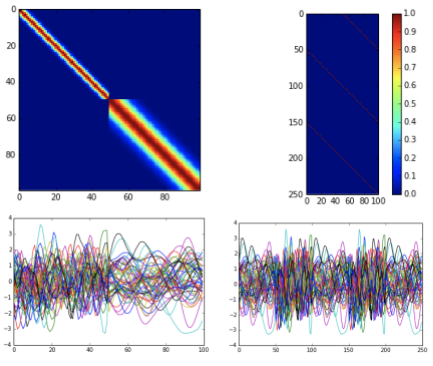
\includegraphics[scale=0.45]{thesis/images/eslfm_data.png}
    \caption{Artificial data set generated for Extended GPBFA: Upper row shows the SE Kernel for latent GP (with shorter and longer length scales) and mixing matrix. Second row demonstrates the actual latent GPs and resulting data generated by mixing them. }
    \label{fig:eslfm_data}
\end{figure}
To demonstrate the ability of extended GPBFA to extract different latent processes inherent in each instance we use an artificially generated dataset in which each instant is obtained by mixing two GPs (Figure \ref{fig:eslfm_data}). For identification purposes  we make one latent GP to have significantly shorter length scale than the other.
\begin{figure}
    \centering
    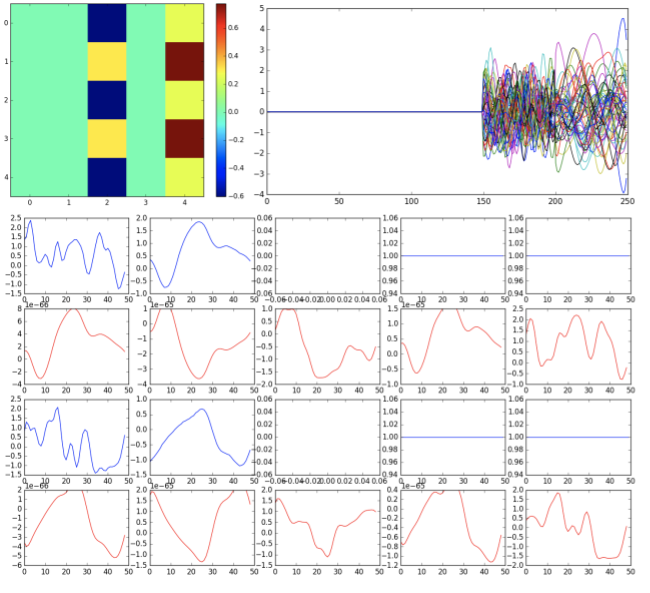
\includegraphics[scale=0.45]{thesis/images/eslfm_demo.png}
    \caption{Extracting latent processes using extended GPBFA: Upper row shows the real latent process (with periodic, linear and Gaussian kernels) and mixing matrix. Second row demonstrates the extracted latent structure using variational inference. Gray Spikes indicate the inducing points at which functions were evaluated}
    \label{fig:eslfm_demo}
\end{figure}
GPs for inference algorithm are initialized randomly with constant lengthscale and random mixing matrix. Figure \ref{fig:eslfm_demo} shows the correctly inferred binary mixing matrix along with redundant processes shut off. We also display comparisons between the actual and inferred latent processes of two random instances in Figure.Please note that all the results were obtained by using only $80\%$ of the data points.


\subsection{Conclusions}
In this section we first reviewed probabilistic linear factor analysis models. The mdoel later described as GPBFA is very similar to [Seeger], however they use IVM framework for inference of latent processes and provide point estimate for mixing matrix. In our treatment  of GPBFA we derived a sparse variational approximation for latent processes which provide complete probability distributions for both latent processes as well as the mixing matrix. Moreover, our experiments with artificial data showed that it our sparse solution is able to recover latent structure by using only half of the actual data thereby making the proposed inference process more scalable and time efficient. [Luttinen's] has a similar approach but also puts a temporal structure on mixing matrix.We further extended the GPBFA model to include multi-trial/instance support and demonstrated that a sparse solution is still capable of recovering separate latent processes from each instance effectively. 





\clearpage
\section{Latent Gaussian Process Classifier}

\thispagestyle{empty}
Expanding on the same idea of separate latent GPs for multiple sequences of each trial, in this section we introduce  a new model that combines a logistic classifier with our extended GPBFA model. This  GP based latent classifier for high dimensional temporal instances proves to be an effective classifier since it not only projects the observations into latent space but also learns a discriminatory plane in that space simultaneously.

\subsection{The Model}

In previous sections we studied models that are able to learn the inherent structure from high dimensional instances of observations, in this model we combine the latent model with a classifier and use a variatioanl algorithm to get closer to the optimal distributions one step at a time. 

Consider observations $ {Y,L}$, where $ Y \in \mathcal{R} S \times C \times N$ and each observational instance $Y[s]$ is associated with a label $L, L \in {-1,1} S \times 1$ signifying it to be in one class or another. 

Conceptually one can imagine that  both data and its labels arise from the same latent space. The discriminatory information about the samples (labels) thus, can be further utilized to learn the most relevant latent space, i.e. the one in which data can be separated best.

\begin{figure}
    \centering
    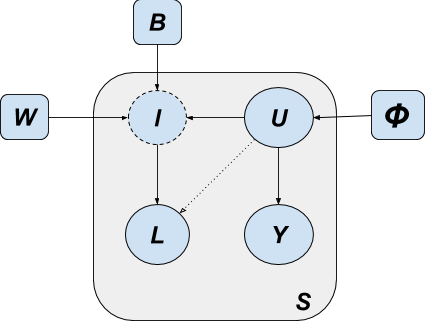
\includegraphics[scale=0.5]{thesis/images/LCMGP_Model.png}
    \caption{Graphical representation of Gaussian Process based latent classifier (lgpc)}
    \label{fig:lgpc}
\end{figure}

As can be seen from figure \ref{fig:lgpc}, 
we introduced a dummy variable $l$  to help  us keep track of classifier values in the latent space. For each data sample $s \in S$, a set of latent processes $u \in U , u \in \mathcal{R}^{P \times N} $ are assumed to generate observed sequence $Y[s] \in \mathcal{R}^{P \times N} $  through mixing matrix $\phi \in \mathcal{R}^{C \times P} $ and a class label $L[s] \in [-1,+1]$. To learn the separation plane in latent space we attach a logistic classifier between $U$ and $L$ such that in additional to $Y, U$ also generates $l  R^1$. Parameters  of classifier are  $W \in R^S$ and a bias term $B$. Values of l then can be converted into class labels through a static rule $ L[s] = \{1 if l[s] > 0,  -1 otherwise\}$. Similar to the model in previous section we vectorize latent and actual observations for computation purposes, making $U \in mathcal{R}^ {S \times CN}, U \in mathcal{R}^ {S \times PN}$, giving the generative model as,




\begin{equation}
Y= U * \bar{\phi}^T + \sigma^2I
\end{equation}

Once again ${  \bar{\phi} = \phi \times I_{N \otimes N} }$ is also a block diagonal of size $CN \times PN$ with $C \times P$ matrix ${\phi}$ on its diagonal. Corresponding latent label values $l$ are generated as, 

\begin{equation}
l= B + U * W^T + s^2I
\end{equation}

and finally the Labels for each data instance  can be generated through the rule {$L[s] = -1$ if $l[s] < \mu L[s] = +1$, otherwise}
Thus combined data gneration model along with priors can be given as,

\begin{equation}
p(W) \approx \mathcal{N}(W \mid 0, I)
\end{equation}
\begin{equation}
p(B) \approx \mathcal{N}(B \mid 0, I)
\end{equation}
\begin{equation}
p(\phi) \approx \mathcal{N}(\phi \mid 0, I)
\end{equation}
\begin{equation}
p(l | U, B, W) \approx \mathcal{N}(l \mid W^{T}U + B, s^2I)
\end{equation}
\begin{equation}
p(L | l) \approx \delta(Ll > \nu)
\end{equation}
Additionally, We put a GP prior on latent variable $ u \in GP(0,\bar{K^p})$ associated with each observational instance where $\bar{K}$ is also a block diagonal of size $PN \times PN$ with co-variance kernels ${K_p \in R ^{N \times N}}$ for each  Gaussian process on diagonals.

Also, just like in previous model we introduce inducing variable $\hat{u} \in \mathcal{R}^{P \times n}$ for latent processes such that  (n < N) to make the GP inference scalabale. $\hat{u}$ has a GP prior as in previous sections. 

We use a variational inference scheme to approximate the posterior $p(W,B,\hat{u},l \mid Y, L)$.

\subsection{Sparse variatioanl approximation in LCGC}

Following inference as sketched in previous sections we introduce variational distribution $q(W,B,l,\hat{u})$ to approximate the posterior. Variational updates for the parameters can be given as,

\begin{equation}
q(\hat{u}) \approx \mathbb{N}(\hat{u} \mid (y\mathbb{E}[\phi] + \mathbb{E}[w]\mathbb{E}[l]\sigma^2 - \mathbb{E}[w]\mathbb{E}[b]\sigma^2){K}_{pNpn}K_{pnpn}^{-1}\Sigma_{u}^{-1}, \hat{\Sigma_{u}^{-1}})
\end{equation}

where $ \hat{\Sigma_{u}} = K_{pnpn}^{-1} + \frac{1}{\sigma^2}{K_{pnpn}^{-1}K_{pnpN}F_uK_{pNpn}K_{pnpn}^{-1}}$ \\
$F_u = \mathbb{E}[\phi^T\phi] + \sigma^2\mathbb{E}[w^Tw] = Var(\phi) + \mathbb{E}[\phi]^T\mathbb{E}[\phi] + Var(w) + \mathbb{E}[w]^T\mathbb{E}[w]$

Using conditional and affine properties of GP we obtain real latent processes as,

\begin{equation}
q(u) \approx \mathbb{N}(\hat{\mu}M, \Sigma_{u|u^{p}} + M\Sigma_{u}M^{T})}
\end{equation}

where $\hat{\mu}_{u}$ is the mean and ${\hat{\Sigma}_{u}}$ variance of $\hat{u}$\\
Also, $\Sigma_{u|u^{p}} = K_{pNpN} - K_{pNpn}K_{pn}^{-1}K_{pnpN}$ and $M = K_{pnpn}^{-1}K_{pNpn}$

Mixing matrix, 
\begin{equation}
q(\phi) \approx \mathbb{N}(\phi \mid (\bar{V}_{\phi} + I)^{-1}\bar{z}_{\phi}, (\bar{V}_{\phi} + I)^{-1})
\end{equation}
where $\bar{V}_{\phi} = \sum_{s}^{S}(<\bar{u}_s><\bar{u}_s>^T$ + I) 
and $\bar{z}_{\phi} = \sum_{s}^{S}<\bar{u}_s>\bar{y}_{s}^T$
such that $x = vec(\bar{x})$ 

label values in the latent space, 
\begin{equation}
q(l_i) \approx \mathbb{T}\mathbb{N}(l_i \mid (\mathbb{E}[w]\mathbb{E}[u] + \mathbb{E}[b], 2*I, l_i < \mu)
\end{equation}
Here $\mathbb{T}\mathbb{N}$ is the truncated normal distribution and $\mu$ the fixed cut off.

Parameter weights for classifier, 

\begin{equation}
q(W) \approx \mathbb{N}(w \mid [F_u+I]^{-1}(\mathbb{E}[u]^T\mathbb{E}[l] - \mathbb{E}[u]^T\mathbb{E}[B]^T,[F_u+I]^{-1})
\end{equation}

where $F_u = \mathbb{E}[U^{T}U]$

Finally the bias term,
\begin{equation}
q(B) \approx \mathbb{N}(B | (\mathbb{E}[l]^T - \mathbb{E}[U]\mathbb{E}[W]^T,I)
\end{equation}

Derivation details of these approximations can be found in Appendix B. 

\subsection{Prediction using LCGC:}
\begin{figure}
    \centering
    \includegraphics[scale=0.75]{thesis/images/LCGC_input.png}
    \caption{Top: Few sample latent processes (red: negative cases, blue: positive) and mixing matrix, Bottom: Resultant output samples from corresponding processes}
    \label{fig:lcpc_input_demo}
\end{figure}

Category prediction for a new observation follows standard GP prediction steps.
For a new data observation Y*, first we project it to the latent space using \ref{eqn:lcgc_latent}.l* in the latent space can be found using predetermined values of weight parameter and bias. Finally, the label L* can be predicted using static rule for $p(L* \mid l*)$ mentioned in \ref{eqn:LCGC_Lgivenl}. However, since we do not know the values in latent space in advance we have to drop all the terms dependent on them form the expressions.

\begin{equation}
q(u^*) \approx \mathbb{N}(u^* \mid (Y^*\mathbb{E}[\phi])K_{pNpn}K_{pnpn}^{-1}\Sigma_{u}^{-1}M, M\Sigma_{u}M^T)
\end{equation}

\begin{equation}
q(l^*) \approx \mathbb{TN}(l^* \mid (Y^*\mathbb{E}[\phi])K_{pNpn}K_{pnpn}^{-1}\Sigma_{u}^{-1}M, M\Sigma_{u}M^T)
\end{equation}

This also means that some information is lost during prediction and hence it might not be as efficient.



\subsection{Demonstration using LCGC}
For demonstration purposes we use an artificial dataset in which our positive classes are genrated through a special latent process that's a combination of linear and gaussian kernels. This gives us a sort of linear trend. Latent processes for the negative classes are generated using simple gaussian kernels. We pass these through a randomly generated mixing matrix to obtain the observation Y and their corresponding labels L (Figure: \ref{fig:lcpc_input_demo}). 
The observations are then split into training data $(Y_train,L_train)$ and test data $(Y^*,L^*)$. 

\begin{figure}
    \centering
    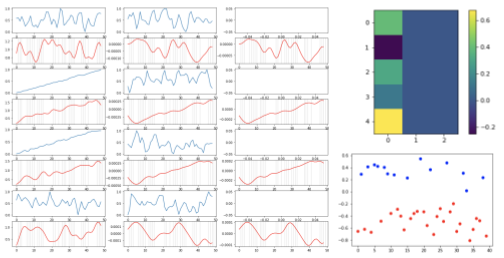
\includegraphics[scale=0.75]{thesis/images/LCGC_output_demo.png}
    \caption{Left: Actual(blue)and extracted(red) latent processes from observed data (vertical lines shows the position of inducing points), Right : Extracted mixing matrix and intermediary variable results on test set}
    \label{fig:lcpc_output_demo}
\end{figure}

To make the inference simple, we used only Gaussian kernel in our GP priors with signal noise ($\sigma = 1$). Figure contains the few extracted latent processes for visual inspection, though we use only $60$ percent of data, we can see that model is able to extract linear trend from the samples. The Gaussian processes are generally ignored due to our assumption of noise to be 1 ($\sigma^2 = 1$), which is also the scale of our observed values. Figure \ref{fig:lcpc_output_demo} also shows the separation of training data in latent space. As can be observed, model is able to achieve a good enough separation of test data in latent space. 
















\clearpage

\section{Experiments and Results}

We tested LCGC model in two different experimental settings. First, we test the impact of different parameters on classification performance using  artificial dataset generated through similar procedure as in previous section. LAter, we use  synthetic control dataset [Reference]  as a benchmark dataset to compare the classification performance of our model against some fundamental classification models.
In a classification setting specially in the scenarios with huge mismatch in number of instances that belong to different categories, accuracy does not provide complete picture and hence we also report F1-Scores as the measure of model’s performance. Reconstruction errors are another important metric which when compared between training and test instances can give us an approximate overview of  over-fitting in the model and thus are reported for the first experiment set. 

\subsection{Artifical data set}

In most of the classification scenarios with multi-series data, number of dimensions in observations (number of sensors for example in sensor data) and sampling resolution (number of samples per sensor) are some important factors that impact predictive performance of models. In this expriment we use an artificial generated dataset to test LCGC's performance  with varying values of output dimension (C) and sampling resolution (N) in datset. Furthermore, we also test model's performance with different number of inducing variable to test model's scalability.
\begin{figure}
    \centering
    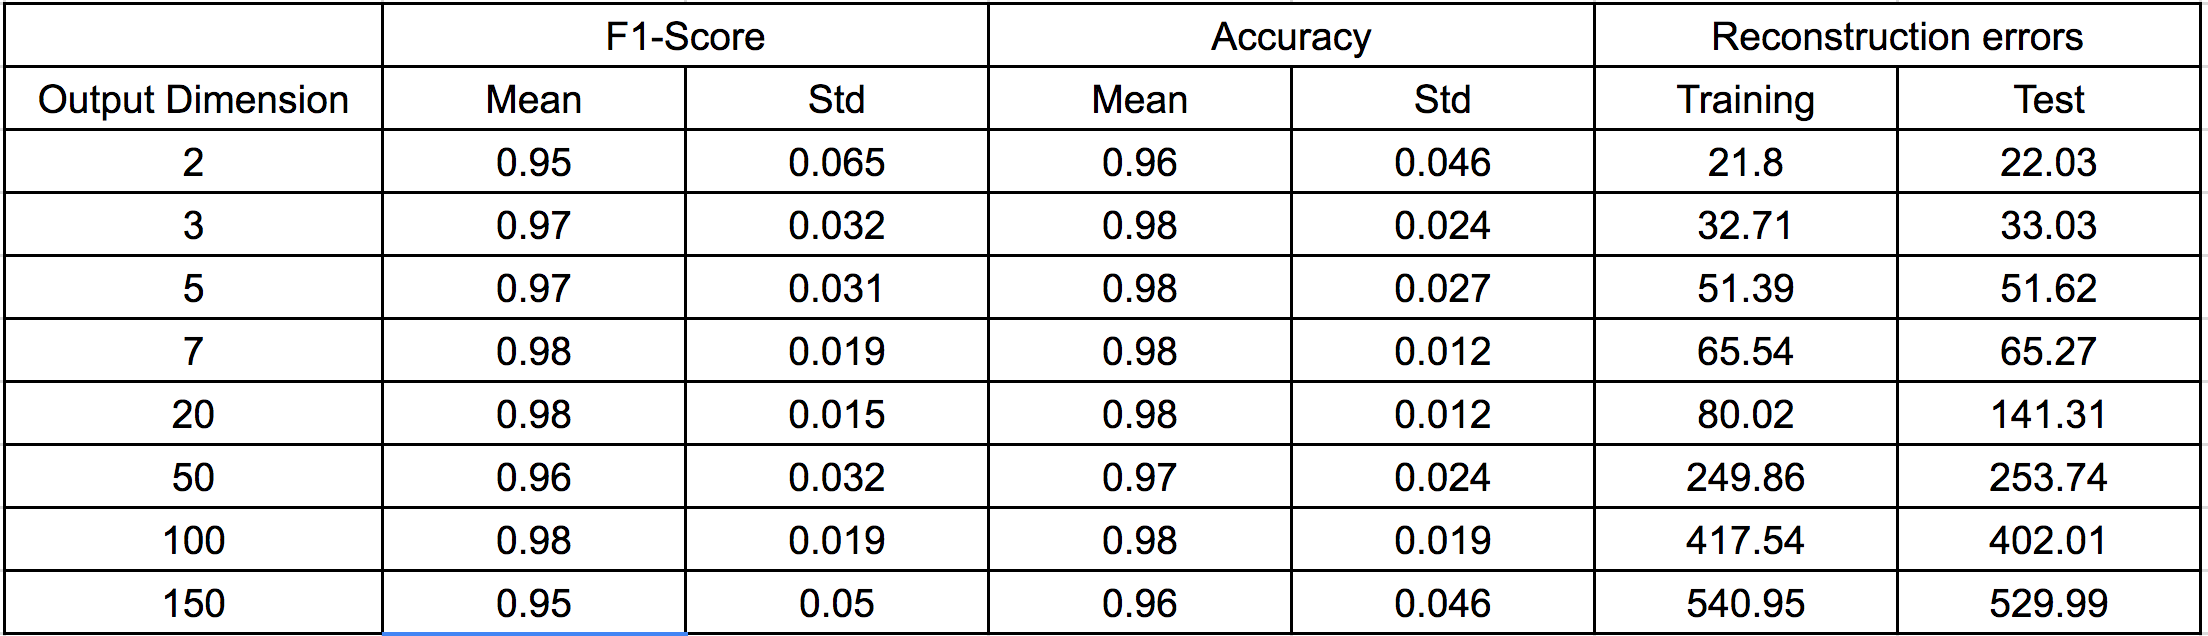
\includegraphics[scale=0.35]{thesis/images/LCGC_output_dimension_results.png}
    \caption{Results of LCGC under different number of output dimensions}
    \label{fig:lcpc_results_C}
\end{figure}
We generated the dataset by mixing two latent  Gaussian processes. For every sample $s \in S$, we mixed either two gaussian processes or one linear and one gaussian process with 40 percent probability. S scaled samples are then generated  by keeping mixing matrix constant throughout the samples. The labels are assigned according to the mixing, i.e. +1 when one of the process has a positive linear slope and  -1 otherwise.

\subsubsection{Effect of output dimensions}
To test the impact of output dimensions, we keep number of latent processes constant (P=2) but change mixing matrix corresponding to a different number of output dimensions. 

Fig \ref{fig:lcpc_results_C} shows our model’s performance with the artificial dataset for different values of C. It’s easy to see that model's performance remain pretty stable even when number of output dimension is near or more than the number of samples. Since model projects data back to a much tighter latent and removes much of redundant columns due to prior on mixing matrix favoring smaller values, number of output dimensions end up losing it's relevance, giving pretty much stable performance over increased number of output dimensions.
\subsubsection{Number of samples}
\begin{figure}
    \centering
    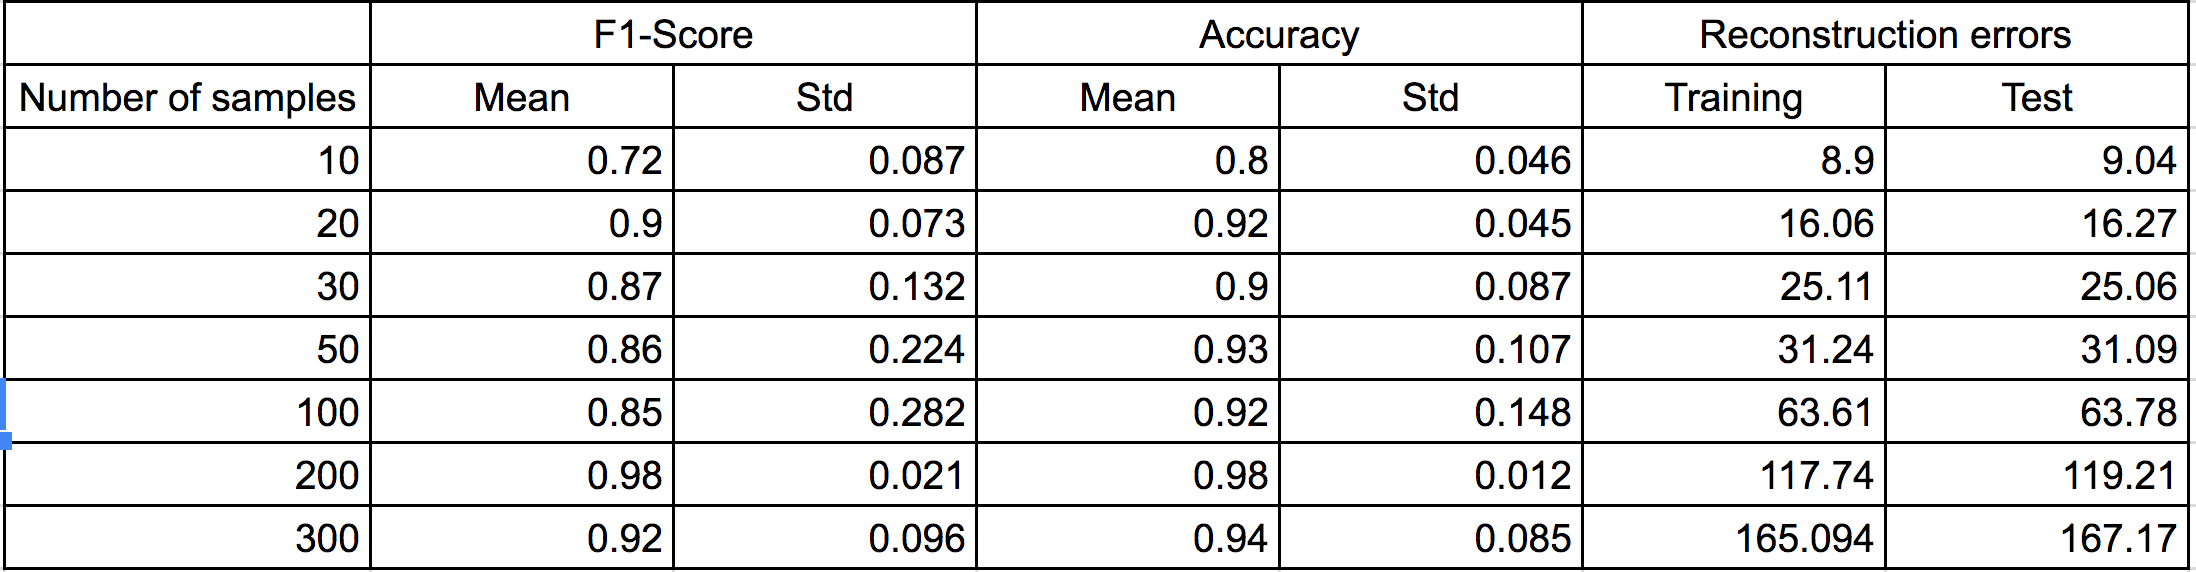
\includegraphics[scale=0.35]{thesis/images/LCGC_samples_results.png}
    \caption{Results of LCGC with varying number of samples in output}
    \label{fig:lcpc_results_samples}
\end{figure}

Fig \ref{fig:lcpc_results_samples} shows us the results when sampling resolution is varied for fixed number of output dimensions (C=3 in this example). Once again we see that model is robust with in a large range of sampling resolution. Even 20 percent of maximum possible samples are enough to yield good enough f1 Scores. Predictive power of course increases as the number of samples available to the model becomes higher.

\subsubsection{Inducing points}
Finally, we also tested classification power of model with different number of inducing points, The ability to use lesser number of inducing points with minimum impact on performance makes the model scalable since sparse solution drastically reduces the time complexity of inference procedure from $O(N^3)$ to $O(Nn^3)$, where $n << N$. 
As evident from the Fig \ref{fig:lcpc_results_induction}, even 50 percent reduction in the number of points is able to achieve good enough classification accuracy on the dataset indicating that huge speed ups are possible with  presented sparse solution of the model.

\begin{figure}
    \centering
    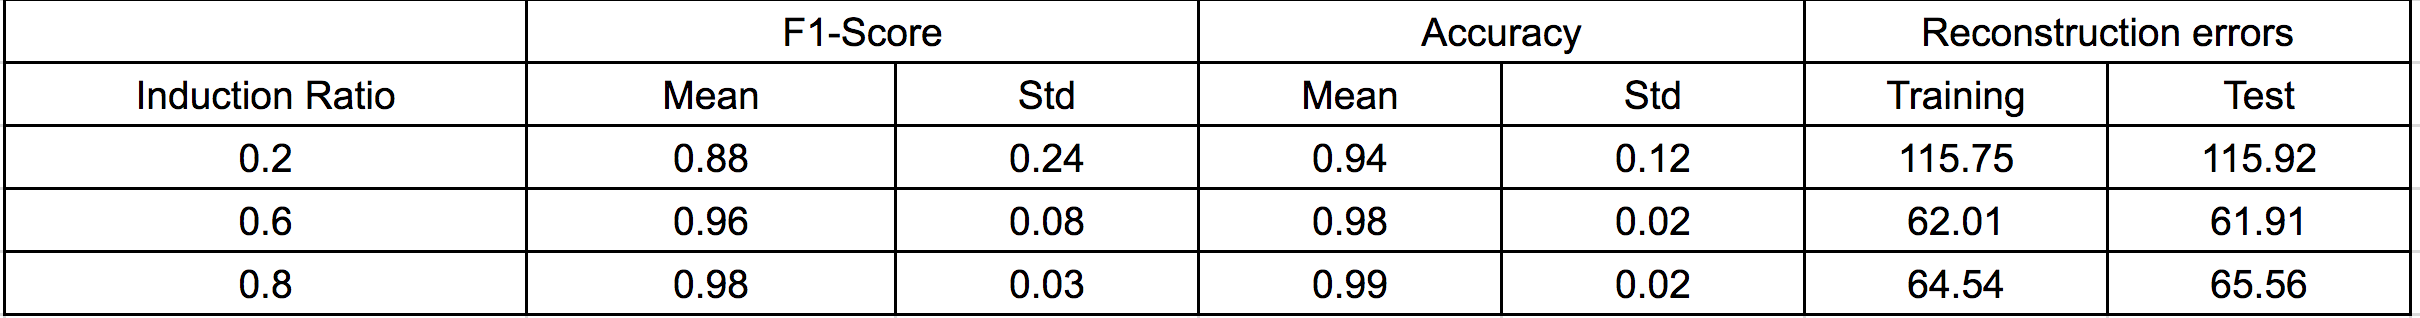
\includegraphics[scale=0.35]{thesis/images/LCGC_inducing_results.png}
    \caption{Results of LCGC under different levels of induction ratio}
    \label{fig:lcpc_results_induction}
\end{figure}
\subsection{Synthetic control dataset}
We use a benchmark dataset namely ‘synthetic control data set’ [1] from UCI to test the classification performance of our  model and then comparing it against other standard classification models. The dataset has a collection of 600 series instances with five different trends: Upward and downward trend, upward and downward shift, cyclic trend and random noise. For the experiment we divide entire datset into training and test instances and try  to predict the correct classification for test data using the parameters learned during training. 
\begin{figure}
    \centering
    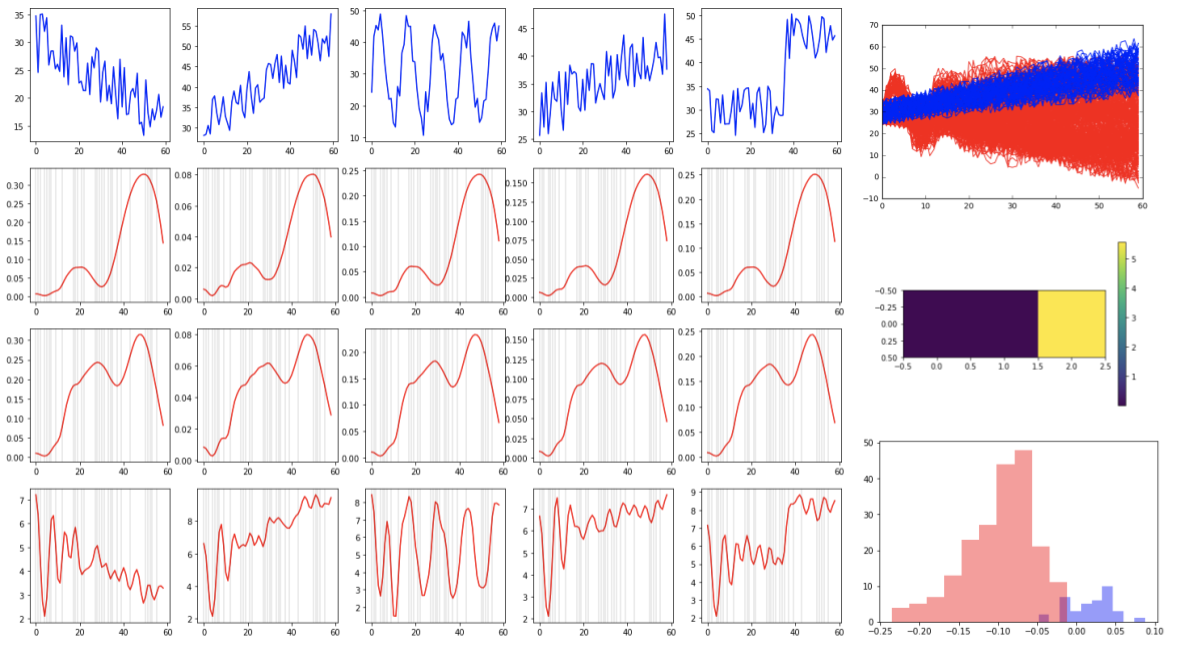
\includegraphics[scale=0.35]{thesis/images/LCGC_real_classification.png}
    \caption{LCGC results on synthetic control dataset: Left: Top rows shows the samples from test dataset, Bottom three rows show respective guessed latent processes. Right top: training dataset with blue showing postive instances, middle: Infered mixing matrix, bottom: Separation inferred among test instances.}
    \label{fig:lcgc_classifications}
\end{figure}
For this experiment, LCGC model was employed with it's default settings (P=3, gaussian Kernels) and 0.8 induction ratio. Top right side of the Figure displays the training dataset with positive classes colored in blue. Rest of the figure shows the result of classification;  mixing matrix in top middle and the guessed latent processes (2-4th row)for few samples of test instances (first row) in the bottom. Top right shows the clear separation between most of the latent values $l*$ of test instances. As we can observe guesses latent processes of LCGC accurately mimic the actual instance thereby decently separating the test instances into their respective classes. 

Moreover, Figure \ref{fig:lcpc_classification_results} shows the comparison between LDA, logistic regression and linear SVM with LCMGP, and we can see that even with 0.8 induction ratio and only default settings performance of LCGC is at par with other time tested algorithms. All of the other classification models were taken from publicly available Scipy implementations[2].
\subsection{Conclusion}
\begin{figure}
    \centering
    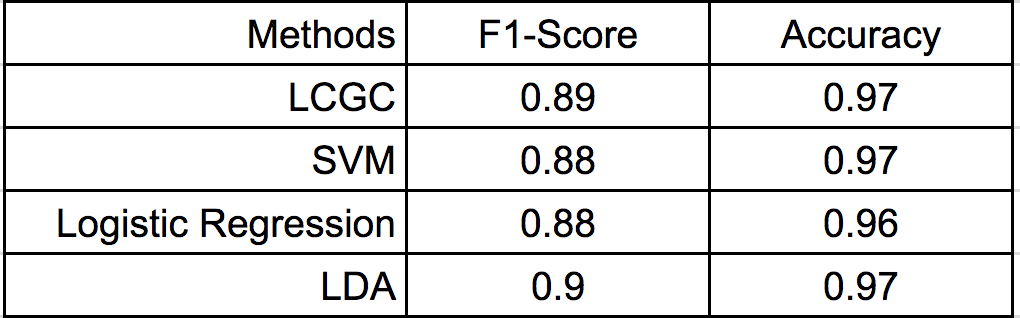
\includegraphics[scale=0.45]{thesis/images/LCGC_classification_results.png}
    \caption{Comparative results of different classification methods on synthetic control dataset }
    \label{fig:lcpc_classification_results}
\end{figure}

Results on artificially generated dataset were promising and indicate that the model's result will be stable under varrying conditions. The results of classification experiment with synthetic control dataset are onpar with the other state of the art classification algorthms, specially considering that a very simple implementation of LCGC was used, optimizations for hyper parmaters as well as inducing point selecition schemes can be used to improve the predictive power of model. The only caveat during experimentation is due to the variational nature of model a specially bad initialization of parameters might stop model from converging within specified number of iterations. These events are however rare and overall results of all of our experiments indicate that LCGC can be a promising model in cases  where the data is generated through a long series of multiple measurements for example in medical, meteorological settings etc.


\clearpage

\section{Conclusions and discussion}
In this section we briefly mention the body of literary work directly adjacent to our contribution and later, we summarize the results and conclusions of this thesis. Finally we also mention few immediate pointers to the future works the thesis might lead to.

\subsection{Related Work}
Model proposed in this thesis assumes that the observations as well as their labels were generated by a linear combination of multiple latent processes. [Luttinen] used a similar approach in probabilistic factor analysis case to model spatio-temporal datasets by using Gaussian process priors for both mixing matrix as well as the latent components corresponding to time signals.  [GPRN] in their model GPRN combine the ideas of Bayesian neural network structure by making the mixing matrix input dependent Gaussian process and thereby introducing non linearity in the mixture as well and created a general purpose multi tasking framework. [Sami’s paper] further extends the idea by proposing a novel non stationary Latent Correlational Kernel that creates a shared correlation structure between the input dependent latent processes. Both regression and classification tasks on multi observational sets are handeled by [Sami’s paper]. 

Another direction of research is the introduction of deeper hierarchy in the latent part of the model. [Neil] proposes an extension to GP-latent variable model which can scale [GPLVM] vertically by encoding multiple layers of latent spaces as well as horizontally by introducing additional conditional independencies between latent variables. 

\subsection{Conclusions}
To summarize, our main objective in this thesis was to present a latent Gaussian processes classifier that is capable of ingesting multivariate data streams for each instance and categorize them in separate classes by extracting the relevant information to a low dimensional latent space. Gaussian processes enable a rich non linear latent space for the data to be projected into, while a sparse solution alleviates the scalability issues that may creep into when using GPs.

Proposed model was tested as a single class classifier in two different experiment settings, first using an artificial dataset where positive instances consisted of a linear trend mixed with other Gaussian trend to test model’s performance with different parameter scenarios like varying amount of output dimensions, induction ratio etc. The results presented in section 3.3.1 of this experiment conclude that the model is stable and classifier performance was consistent. Second experiment was performed using an open source benchmark dataset for time series from UCI, to test model’s performance in a more real setting and compare it with other classification methods. Results of this experiment as explained in section 3.3.2 were also very promising and demonstrated that the performance of LCGC with a default settings was comparable to the open source implementation of other state of the art classification methods like Logistic regression, SVM etc. Moreover, being a fully Bayesian model, using LCGC also means that uncertainty information is readily available at every stage of inference be it latent processes or latent predicted values something that’s not possible with above mentioned models.

In addition to proposing LCGC, we also extended SLFM model proposed by [Seeger et al] by enabling it to handle multi-observational scenarios such that each observation has it's own latent space and proposing a sparse variational approximation both to original model as well as our extension of it. As explained in section 1.3, computational complexity of inference in Gaussian process grows with an order of three which can make working with large dataset challenging. Sparse solution thus makes the model more scalable and efficient. Visual demonstrations of these models on artificially generated datasets provided in section 2.2.3 and 2.3.2 respectively indicate that the sparse models are able to satisfactorily capture the latent processes of data even with a 0.5 to 0.7 induction ratio.

The experiments and demonstrations in this thesis were performed only on artificially generated or simulated datasets, hence an immediate future continuation of this work might include the tests and experiments based on real world datasets. Apart from classical FMRI, share recognition datasets many new datasets should be expected following the recent explosion of data collection in IoT as well as wearable device and medical areas. Moreover, all of the experiments the naïve LCGC model was used with default Gaussian kernels for latent processes. In real world however, there is always much more information about the supposed latent structure is available. This information can be encoded in the model by using different types of Kernel in the latent processes, for example a periodic or Brownian model might provide better results if the data is known to have cycles or trends structures. Similarly, performing hyper-parameter optimization before variational algorithm should also help improve the performance of LCGC model in real world data analysis problems. 





\clearpage
%% L\"ahdeluettelo
%%
%% \phantomsection varmistaa, ett\"a hyperref-paketti latoo hypertekstilinkit
%% oikein.
%%
%% The \phantomsection command is nessesary for hyperref to jump to the 
%% correct page, in other words it puts a hyper marker on the page.

\phantomsection
\addcontentsline{toc}{section}{\refname}
%\addcontentsline{toc}{section}{References}
\begin{thebibliography}{99}

%% Alla pilkun j\"alkeen on pakotettu oikea v\"ali \<v\"alily\"onti>-merkeill\"a.
\bibitem{Kauranen} Kauranen,\ I., Mustakallio,\ M. ja Palmgren,\ V.
  \textit{Tutkimusraportin kirjoittamisen opas opinn\"aytety\"on
    tekij\"oille.}  Espoo, Teknillinen korkeakoulu, 2006.

\bibitem{Itkonen} Itkonen,\ M. \textit{Typografian k\"asikirja.} 3.\
  painos.  Helsinki, RPS-yhti\"ot, 2007.

\bibitem{Koblitz} Koblitz,\ N. \textit{A Course in Number Theory and
    Cryptography. Graduate Texts in Mathematics 114.}  2.\ painos. New
  York, Springer, 1994.

%% Kun on useampi nimikirjain, jokaisen nimikirjaimen v\"aliin
%% kuuluu v\"alily\"onti. Oikea v\"alin m\"a\"ar\"a on saatu \<v\"alily\"onnill\"a>
\bibitem{bcs} Bardeen,\ J., Cooper,\ L.\ N. ja Schrieffer,\ J.\ R.
  Theory of Superconductivity. \textit{Physical Review,} 1957, vol.\
  108, nro~5, s.\ 1175--1204.

\bibitem{Deschamps} Deschamps,\ G.\ A. Electromagnetics and
  Differential Forms. \textit{Proceedings of the IEEE,} 1981, vol.\
  69, nro~6, s.\ 676--696.

%% Alla esimerkki englanninkielisen tavuttamisen pakottamisesta.
%% Oletusarvoisesti k\"aytet\"a\"an suomalaista tavutusta, mutta viitteiss\"a
%% esiintyy usein muunkielisi\"a lauseita, jotka tulevat siten tavutetuksi
%% suomen kielen s\"a\"ant\"ojen mukaan. T\"am\"an voi korjata \foreignlanguage-
%% komennolla, jonka ensimm\"ainen parametri on vieraan kielen nimi ja toinen 
%% on vieraalla kielell\"a tavutettava teksti. 
\bibitem{Sihvola} Sihvola,\ A.\ et al.
  \foreignlanguage{english}{Interpretation of measurements of helix 
    and bihelix superchiral structures.}
  Teoksessa: Jacob,\ A.\ F. ja
  Reinert,\ J. (toim.) \textit{Bianisotropics '98 7th International
    Conference on Complex Media.}  Braunschweig, 3.--6.6.1998.
  Braunscweig, Technische Universit\"at Braunschweig, 1998, s.\
  317--320.

%% Alla on suomalainen yhdistelm\"asukunimi. Sen nimien v\"aliss\"a 
%% k\"aytet\"a\"an yhdysmerkki\"a l. tavuviivaa, kirjoitetaan -.
\bibitem{Lindblom} Lindblom-Yl\"anne,\ S. ja Wager,\ M.  Tieteellisten
  opinn\"aytet\"oiden ohjaaminen. Teoksessa: Lindblom-Yl\"anne,\ S. ja
  Nevgi,\ A. (toim.) \textit{Yliopisto- ja korkeakouluopettajan
    k\"asikirja.}  Helsinki, WSOY, 2004, s.\ 314--325.
 
\bibitem{Miinusmaa} Miinusmaa,\ H. Neliskulmaisen rei\"an poraamisesta
  kolmikulmaisella poralla. Diplomity\"o, Teknillinen korkeakoulu,
  konetekniikan osasto, Espoo, 1977.

%% T\"ass\"a taas pakotettu englanninkielinen tavutus. 
%% Pedanttinen kirjoittaja pakottaa tietysti jokaiseen englanninkieliseen
%% lauseeseen englannin tavutuksen, mutta t\"ass\"a esityksess\"a ei n\"ain ole
%% tehty selvyyden ja l\"ahdekoodin luettavuuden takia. 
\bibitem{Loh} Loh,\ N.\ C. High-Resolution Micromachined
  Interferometric Accelerometer. Master's Thesis, Massachusetts
  Institute of Technology, Cambridge,
  \foreignlanguage{english}{Massachusetts,} 1992.

\bibitem{Lonnqvist} L\"onnqvist,\ A.
  \foreignlanguage{english}{Applications of hologram-based compact
    range: antenna radiation pattern, radar cross section, and
    absorber reflectivity measurements.}
  V\"ait\"oskirja, Teknillinen korkeakoulu, s\"ahk\"o- ja tietoliikennetekniikan
  osasto, 2006.

\bibitem{sfs} SFS 5342. Kirjallisuusviitteiden laatiminen. 2.\ painos.
  Helsinki, Suomen standardisoimisliitto, 2004. 20~s.

\bibitem{haastattelu} Palmgren,\ V. Suunnittelija. Teknillinen
  korkeakoulu, kirjasto. Otaniementie 9, 02150 Espoo. Haastattelu
  15.1.2007.

\bibitem{Ribeiro} Ribeiro,\ C.\ B., Ollila,\ E. ja Koivunen,\ V.
  \foreignlanguage{english}{Stochastic Maximum-Likelihood Method for
    MIMO Propagation Parameter Estimation.}
 \textit{IEEE Transactions
    on Signal Processing,} verkkolehti, vol.\ 55, nro~1, s.\ 46--55.
  Viitattu 19.1.2007. Lehti ilmestyy my\"os painettuna. DOI:
  10.1109/TSP.2006.882057.

\bibitem{Stieber} Stieber,\ T. GnuPG Hacks. \textit{Linux Journal,}
  verkkolehti, 2006, maaliskuu, nro~143. Viitattu 19.1.2007. Lehti
  ilmestyy my\"os painettuna. Saatavissa:
  \url{http://www.linuxjournal.com/article/8732.}

\bibitem{kone} Pohjois-Koivisto,\ T. Voiko kone tulevaisuudessa arvata
  tahtosi?  \textit{Apropos,} verkkolehti, helmikuu, nro~1, 2005.
  Viitattu 19.1.2007.  Saatavissa:
  \url{http://www.apropos.fi/1-2005/prima.php.}

\bibitem{Adida} Adida,\ B.  Advances in Cryptographic Voting Systems.
  Verkkodokumentti. Ph.D.\ Thesis, Massachusetts Institute of
  Technology, Cambridge, 
  \foreignlanguage{english}{Massachusetts,}
  2006. Viitattu 19.1.2007.  Saatavissa:
  \url{http://crypto.csail.mit.edu/~cis/theses/adida-phd.pdf.}

\bibitem{viittaaminen} Kilpel\"ainen,\ P. WWW-l\"ahteisiin viittaaminen
  tutkielmatekstiss\"a. Verkkodokumentti. P\"aivitetty 26.11.2001.
  Viitattu 19.1.2007. Saatavissa:
  \url{http://www.cs.uku.fi/~kilpelai/wwwlahteet.html.}

\end{thebibliography}

%% Appendices
%% Liitteet
\clearpage

\thesisappendix

\section{Details of GP based factor analysis posterior inference \label{AppendixA}}

In order to make the posterior computationally tractable, we introduce another distribution $\hat{u_p}$ which is evaluated over fewer values than the original $u_p$. Thus posterior distribtion $p(\phi,u,\hat{u} \mid Y)$ is approximated as a factorized distribution given by:
$${ q(\phi,u, \hat{u}) = q(\phi)\prod_{p=1}^{P}p(u|\hat{u_p})q(\hat{u_p}) }$$


After introducing sparse variational approximations and taking log both sides of marginal likelihood of the observations,  equation \ref{eqn:gpfa_lklihd}  can be written as, 
\begin{equation}
   L(Y|X) = \int q(\phi) \prod_{p=1}^{P}{p(u_p|\hat{u_p})q(\hat{u}_p)} \log \frac{p(Y|\hat{u},\phi) p(\phi)\prod_{p=1}^{P}p(\hat{u_p})}{q(\phi)\prod_{p=1}^{P}q(\hat{u_p})}  d\phi d\hat{u}
    \label{eqn:gpfa:liklehood_complete}
\end{equation}

rewriting above equation in terms of $\hat{u_p}$,

\begin{equation}
L(\hat{u}_p) = \int q(\hat{u}_p) log \frac{\bar{p}(Y|\phi,\hat{u}_p)p(\hat{u}_p)}{\hat{u}_p}
\label{eqn:u_pfactorized}
\end{equation}
where,
\begin{multiline}
    \begin{split}
        \log \bar{p}(Y|\phi,\hat{u}_p) = & \int q(\phi) p(u_p \mid \hat{u_p}) \prod_{i=1}^{P\backslash  p}{p(u_i\mid\hat{u_i})q(u_i)} \log p(Y \mid \hat{u},\phi) d\phi d\hat{u}_{1....P\p} \\
        & -\sum_{i=1}^{P \backslash p}{KL(q(\hat{u_i}\mid\mid p(\hat{u_i}))} - KL(q(\phi)\mid\mid p(\phi))
    \end{split}
\end{multiline}


Now, we can factorizing Y over it's row, i.e. C's,

\begin{equation}
\log \bar{p}(Y|\phi,\hat{u}_p) = \sum_{c}^{C} <log(Y_c|\phi_c,u)>_{\phi,p_{1..P\backslash p},u_p|\hat{u}_p}  - KLs
\end{equation}

After expanding the terms and completing the square we can obtain following parameterization:

\begin{equation}
\log \bar{p}(Y|\phi,\hat{u}_p) = \log N ({S}_{p}^{-1}z_p| K_{Nn}K_{n}^{-1}\hat{u}_p, K_{N} - K_{Nn}K_{n}^{-1}K_{nN}) - \frac{1}{2}tr(\sum_{i}^{P}{S_i*cov(u_i|\hat{u_i}}))   - KLs
\end{equation}
where $$z_p = \sum_{c}^{C}\mathbb{E}[\phi_{cp}](y_c - \sum_{i}^{P/p}\mathbb{E}[\phi_{ci}]\mathbb{E}[u_{ip}]),$$ 
and $$S_p = \sum_{c}^{C}\mathbb{E}[\phi_{cp}^2]$$

Substituting this back in the equation \ref{eqn:u_pfactorized},

\begin{multiline}
L(\hat{u}_p) = \int q(\hat{u_p}) \log \frac{ N ({S}_{p}^{-1}z_p \mid K_{Nn}K_{n}^{-1}\hat{u}_p, K_{NN} - K_{Nn}K_{nn}^{-1}K_{nN}) p(\hat{u}_p)}{q(u_p)}  - \frac{1}{2}tr(\sum_{i}^{P}{S_i*cov(u_i\mid \hat{u_i}}))   - KLs 
\label{eqn:up_maximized}
\end{multiline}

Above equation can be used for hyperparmater selection however to find the optimal distribution $q(\hat{u_p})$ one can discard the constant terms and use only the lower bound:
\begin{equation}
L(\hat{u}_p) \geq \int q(\hat{u_p}) \log \frac{ \matchal{N} ({S}_{p}^{-1}z_p \mid K_{Nn}K_{n}^{-1}\hat{u}_p, K_{NN} - K_{Nn}K_{nn}^{-1}K_{nN}) p(\hat{u}_p)}{q(u_p)}
\label{eqn:up_variational_bound}
\end{equation}

The ELBO obtained above can be interpreted as the KL distance between variational distribution of $\hat{u_p}$ and the nominator value. This distance naturally is minimal when denominator $\hat{u_p}$ takes the value same as the nominator, i.e.

\begin{equation}
q(\hat{u}_p) \approx  \matchal{N} ({S}_{p}^{-1}z_p \mid K_{Nn}K_{n}^{-1}\hat{u}_p, K_{NN} - K_{Nn}K_{nn}^{-1}K_{nN}) p(\hat{u}_p)
\end{equation}

Rearranging terms
\begin{equation}
q(\hat{u}_p) \approx N(\Sigma_{p}^{-1}K_{nn}^{-1}K_{Nn}z_p,\Sigma_{p}^{-1})}$$
where $${\Sigma_{p} = K_{n}^{-1} + \frac{1}{\sigma^2}K_{n}^{-1}K_{nN}S_pK_{Nn}K_{n}^{-1}
\label{eqn:slfm_u_hat}
\end{equation}

Note: More rigorous ways to reach at identical optimal distribution using variational calculus or by reversing Jensen's equality can be found in [https://arxiv.org/pdf/1402.1412.pdf] and [Tistia 09 tech report] respectively. 

Moreover,  we know that , $${q(u_p) = \int p(u_p \mid \hat{u_p})q(\hat{u_p})d\hat{u_p}}$$
where factor $p(u_p \mid \hat{u_p})$ can be easily obtained through conditional of GP priors $u_p$ and $\hat{u_p}$. Using affine property of gaussians [Bishop pg 87-89] and equation \ref{eqn:slfm_u_hat} we can obtain,

$${
q(u_p) \approx \mathcal{N}(u_p \mid M\hat{\mu_{p}}, \Sigma_{u \mid \hat{u}}^{p}} + M\Sigma_pM^T)
}$$
where ${\hat{\mu_{p}}$ is the mean of GP $\hat{u_p}$, ${M = K_{Nn}K_{nn}^{-1} }$ and
${\Sigma_{u\mid\hat{u}}^{p}} = K_{NN} - MK_{nN} }$

An optimization process similar to $\hat{u_p}$ can be followed to find the lower bound with respect to $\phi$,i.e.

\begin{equation}
L(\phi) = \int q(\phi) \log\frac{\bar{p}(Y|\phi,u)p(\phi)}{q(\phi) } d\phi
\label{eqn:phi_maximized}
\end{equation}

where $${\log \bar{p}(Y|\phi,u) = \int q(u) log \frac{p(Y|\phi,u)p(u)}{q(u)} du \\ = \int q(u) \log {p(Y|\phi,u)} du - KL(q(u)|| p(u)) }$$

Variational distribution is given by, 

$${q(\phi) \approx \mathcal{N}(\phi \mid y\mathbb{E}[U]^T\Sigma_{\phi}^{-1}, \Sigma_{\phi}^{-1})}$$
where ${\Sigma_{\phi} = (V_{\phi}^{-1} + I )}$
and ${V_{\phi} = \mathbb{E}[u]\mathbb{E}[u]^T\sigma^2}$



\clearpage
\section{Details of LGPC posterior \label{AppendixB}}

Joint distribution of LGPC (Figure \ref{fig:lgpc}) can be given by,
 
$$p(L,Y, l, B, W, U, \sigma^2,\phi) = p(W)p(B)p(L \mid l)p(l \mid B, W, U)p(Y \mid U, \phi, \sigma^2)p(U)p(\phi)$$

The data likelihood can be given as, 

\begin{equation}
p(L,Y) = \mathlarger{\int} p(W)p(B)p(L \mid l)p(l \mid B, W, U)p(Y \mid U, \phi, \sigma^2)p(U)p(\phi) dW dB dU d\phi dl
\label{eqn:lgpc_likelihood}
\end{equation}


Now We introduce a factorized  variational distribution $q(W,B,U, l, \phi)$ to approximate the posterior $p(W,B,U , l , \phi \mid Y, L)$, i.e,
\begin{equation}
  $p(W,B,U, l \mid Y, L)$ \approx $q(W,B,u, l)$
  \approx q(W)q(B)q(U)q(\phi)q(l)
\end{equation}

Additionally to make the inference scalable, a sparse approximation $\hat{U}$ is put in place of $U$ such that $q(U) \approx p(U \mid \hat{U}) q(\hat{U})$. This further factorizes the variational distributoin as,
\begin{equation}
    q(W,B,U,\phi, l) \approx q(W)q(B)p(U \mid \hat{U})q(\hat{U})q(\phi)q(l)
\end{equation}

Now we use this to rewrite the likelihood equation \ref{eqn:lgpc_likelihood},
\begin{equation}
\mathbb{L}(L,Y) = \mathlarger{\int} q(W)q(B)p(U \mid \hat{U})q(\hat{U})q(\phi) \log \frac{p(W)p(B)p(L \mid l)p(l \mid B, W, U)p(Y \mid U, \phi, \sigma^2)p(\hat{U})p(\phi)}{q(W)q(B)q(\hat{U})q(\phi)q(l)} dW dB d\hat{U} d\phi dl
\label{eqn:lgpc_likelihood}
\end{equation}
The update for $\hat{U}$ is derived by rewriting the likelihood equation as, 
\begin{equation}
\mathbb{L}(L,Y) = \mathlarger{\int} q(\hat{U}) \log \frac{\bar{p}(L,Y \mid \hat{U})p(\hat{U})}{q(\hat{U})}  d\hat{U} 
\label{eqn:lgpc_likelihood_reWrtn}
\end{equation}
and, 
\begin{equation}
log \bar{p}(L,Y \mid \hat{U}) = \mathlarger{\int} q(W)q(B)p(U \mid \hat{U})q(\phi) \log \frac{p(W)p(B)p(L \mid l)p(l)p(l \mid B, W, U)p(Y \mid U, \phi, \sigma^2)p(\phi)}{q(W)q(B)q(\phi)q(l)} dW dB d\hat{U} d\phi dl
\end{equation}

Separating log and KL divergence terms,

\begin{equation}
= \mathlarger{\mathbb{E}[ log \mathcal{N}(l \mid B, W, U) + log \mathcal{N}(Y \mid U, \phi, \sigma^2) ]_{W,B,l,\phi} } - KL(\phi,W,B,l) 
\end{equation}

Here $KL(\phi,W,B,l)$ represent the KL divergence between their true and posterior approximations. 
Expanding the terms inside the expectations and rearranging them we obtain, 
\begin{equation}
log  \bar{p}(L,Y \mid \hat{U}) = \mathlarger{\int q(W)q(B)p(U \mid \hat{U})q(\phi) \log   \frac{p(W)p(B)p(L \mid l)p(l)p(l \mid B, W, U)p(Y \mid U, \phi, \sigma^2)p(\phi)}{q(W)q(B)q(\phi)q(l)} dW dB d\hat{U} d\phi dl
\end{equation}

Which after expanding the normal and rearranging few terms can be written as:

\begin{equation}
 log  \bar{p}(L,Y \mid \hat{U}) = log \mathcal{N}(F_{u}^{-1}[\mathbb{E}[W]\mathbb{E}[l]\sigma^2 + Y\mathbb{E}[\phi] - \mathbb{E}[W]\mathbb{E}[B]\sigma^2] \mid \mathbb{E}[U]^T, F_{u}^{-1}) - \frac{Tr}{2}[Cov(L|l, l) + Cov(U|\hat{U}\mathbb{E}[W^TW]) + Cov(U|\hat{U})\mathbb{E}[\phi^T\phi] + Cov(B) ]
\end{equation}

additionally we can ignore $p(L \mid l)$ in expectations since it will always be a constant.   





\end{document}